%% LyX 2.4.0~RC3 created this file.  For more info, see https://www.lyx.org/.
%% Do not edit unless you really know what you are doing.
\documentclass[journal,article,submit,pdftex,moreauthors]{Definitions/mdpi}
\usepackage[utf8]{inputenc}
\usepackage{float}
\usepackage{varwidth}
\usepackage{amsmath}
\usepackage{graphicx}

\makeatletter

%%%%%%%%%%%%%%%%%%%%%%%%%%%%%% LyX specific LaTeX commands.

\Title{Constructing artificial features with Grammatical Evolution for the
motor symptoms of Parkinson’s Disease}

\TitleCitation{Constructing artificial features with Grammatical Evolution for the
motor symptoms of Parkinson’s Disease}

\Author{Aimilios Psathas$^{1}$, Ioannis G. Tsoulos$^{2,*}$, Nikolaos Giannakeas$^{3}$,
Alexandros Tzallas$^{4}$ and Vasileios Charilogis$^{5}$}

\AuthorNames{Psathas, A., Tsoulos, I.G., Giannakeas N, Tzallas, A. \textbackslash\&
Charilogis, V. }

\AuthorNames{Aimilios Psathas, Ioannis G. Tsoulos, Nikolaos Giannakeas, Alexandros
Tzallas and Vasileios Charilogis. }

\AuthorCitation{Psathas, A.; Tsoulos, I.G.; Giannakeas, N.; Tzallas, A.; Charilogis,
V. }


\address{$^{1}$\quad{}Department of Informatics and Telecommunications,
University of Ioannina, Greece;pint00141@uoi.gr\\
$^{2}$\quad{}Department of Informatics and Telecommunications, University
of Ioannina, Greece; itsoulos@uoi.gr\\
$^{3}\quad$Department of Informatics and Telecommunications, University
of Ioannina, Greece; giannakeas@uoi.gr\\
$^{4}\quad$Department of Informatics and Telecommunications, University
of Ioannina, Greece; tzallas@uoi.gr\\
$^{5}\quad$Department of Informatics and Telecommunications, University
of Ioannina, Greece; v.charilog@uoi.gr}


\corres{Correspondence: itsoulos@uoi.gr}


\abstract{This study proposes a new methodology for evaluating Parkinson's
Disease (PD) motor symptoms through complex motion analysis, with
particular emphasis on symptom variations in the periods leading up
to and after medication intake. Data were collected through a custom-made
SmartGlove system during four standardized hand motor tests. An exhaustive
set of features was extracted from the sensor signals, encompassing
essential aspects of motor impairment, such as tremor, bradykinesia,
rigidity, and movement abnormality. An original multi-method scoring
procedure was adopted, combining statistical significance, model-based
importance, and variance contribution, in order to determine the most
discriminative biomarkers while maintaining the top - ranked features
in the top 80\%. The crux of this paper is an assessment of the contribution
of creating synthetic features based on Grammatical Evolution from
the selected subset.}


\keyword{Machine learning; Evolutionary algorithms; Genetic Programming; Grammatical
Evolution}

\DeclareTextSymbolDefault{\textquotedbl}{T1}
%% Because html converters don't know tabularnewline
\providecommand{\tabularnewline}{\\}
%% Variable width box for table cells
\newenvironment{cellvarwidth}[1][t]
    {\begin{varwidth}[#1]{\linewidth}}
    {\@finalstrut\@arstrutbox\end{varwidth}}

%%%%%%%%%%%%%%%%%%%%%%%%%%%%%% Textclass specific LaTeX commands.
\newenvironment{lyxcode}
	{\par\begin{list}{}{
		\setlength{\rightmargin}{\leftmargin}
		\setlength{\listparindent}{0pt}% needed for AMS classes
		\raggedright
		\setlength{\itemsep}{0pt}
		\setlength{\parsep}{0pt}
		\normalfont\ttfamily}%
	 \item[]}
	{\end{list}}

%%%%%%%%%%%%%%%%%%%%%%%%%%%%%% User specified LaTeX commands.
%  LaTeX support: latex@mdpi.com 
%  For support, please attach all files needed for compiling as well as the log file, and specify your operating system, LaTeX version, and LaTeX editor.

%=================================================================
%\documentclass[preprints,article,submit,pdftex,moreauthors]{Definitions/mdpi} 
% For posting an early version of this manuscript as a preprint, you may use "preprints" as the journal. Changing "submit" to "accept" before posting will remove line numbers.

% Below journals will use APA reference format:
% admsci, behavsci, businesses, econometrics, economies, education, ejihpe, famsci, games, humans, ijcs, ijfs, journalmedia, jrfm, languages, psycholint, publications, tourismhosp, youth

% Below journals will use Chicago reference format:
% arts, genealogy, histories, humanities, jintelligence, laws, literature, religions, risks, socsci

%--------------------
% Class Options:
%--------------------
%----------
% journal
%----------
% Choose between the following MDPI journals:
% accountaudit, acoustics, actuators, addictions, adhesives, admsci, adolescents, aerobiology, aerospace, agriculture, agriengineering, agrochemicals, agronomy, ai, air, algorithms, allergies, alloys, amh, analytica, analytics, anatomia, anesthres, animals, antibiotics, antibodies, antioxidants, applbiosci, appliedchem, appliedmath, appliedphys, applmech, applmicrobiol, applnano, applsci, aquacj, architecture, arm, arthropoda, arts, asc, asi, astronomy, atmosphere, atoms, audiolres, automation, axioms, bacteria, batteries, bdcc, behavsci, beverages, biochem, bioengineering, biologics, biology, biomass, biomechanics, biomed, biomedicines, biomedinformatics, biomimetics, biomolecules, biophysica, biosensors, biosphere, biotech, birds, blockchains, bloods, blsf, brainsci, breath, buildings, businesses, cancers, carbon, cardiogenetics, catalysts, cells, ceramics, challenges, chemengineering, chemistry, chemosensors, chemproc, children, chips, cimb, civileng, cleantechnol, climate, clinbioenerg, clinpract, clockssleep, cmd, cmtr, coasts, coatings, colloids, colorants, commodities, complications, compounds, computation, computers, condensedmatter, conservation, constrmater, cosmetics, covid, crops, cryo, cryptography, crystals, csmf, ctn, curroncol, cyber, dairy, data, ddc, dentistry, dermato, dermatopathology, designs, devices, diabetology, diagnostics, dietetics, digital, disabilities, diseases, diversity, dna, drones, dynamics, earth, ebj, ecm, ecologies, econometrics, economies, education, eesp, ejihpe, electricity, electrochem, electronicmat, electronics, encyclopedia, endocrines, energies, eng, engproc, ent, entomology, entropy, environments, epidemiologia, epigenomes, esa, est, famsci, fermentation, fibers, fintech, fire, fishes, fluids, foods, forecasting, forensicsci, forests, fossstud, foundations, fractalfract, fuels, future, futureinternet, futureparasites, futurepharmacol, futurephys, futuretransp, galaxies, games, gases, gastroent, gastrointestdisord, gastronomy, gels, genealogy, genes, geographies, geohazards, geomatics, geometry, geosciences, geotechnics, geriatrics, glacies, grasses, greenhealth, gucdd, hardware, hazardousmatters, healthcare, hearts, hemato, hematolrep, heritage, higheredu, highthroughput, histories, horticulturae, hospitals, humanities, humans, hydrobiology, hydrogen, hydrology, hygiene, idr, iic, ijerph, ijfs, ijgi, ijmd, ijms, ijns, ijpb, ijt, ijtm, ijtpp, ime, immuno, informatics, information, infrastructures, inorganics, insects, instruments, inventions, iot, j, jal, jcdd, jcm, jcp, jcs, jcto, jdad, jdb, jeta, jfb, jfmk, jimaging, jintelligence, jlpea, jmahp, jmmp, jmms, jmp, jmse, jne, jnt, jof, joitmc, joma, jop, jor, journalmedia, jox, jpbi, jpm, jrfm, jsan, jtaer, jvd, jzbg, kidney, kidneydial, kinasesphosphatases, knowledge, labmed, laboratories, land, languages, laws, life, lights, limnolrev, lipidology, liquids, literature, livers, logics, logistics, lubricants, lymphatics, machines, macromol, magnetism, magnetochemistry, make, marinedrugs, materials, materproc, mathematics, mca, measurements, medicina, medicines, medsci, membranes, merits, metabolites, metals, meteorology, methane, metrics, metrology, micro, microarrays, microbiolres, microelectronics, micromachines, microorganisms, microplastics, microwave, minerals, mining, mmphys, modelling, molbank, molecules, mps, msf, mti, multimedia, muscles, nanoenergyadv, nanomanufacturing, nanomaterials, ncrna, ndt, network, neuroglia, neurolint, neurosci, nitrogen, notspecified, nursrep, nutraceuticals, nutrients, obesities, oceans, ohbm, onco, oncopathology, optics, oral, organics, organoids, osteology, oxygen, parasites, parasitologia, particles, pathogens, pathophysiology, pediatrrep, pets, pharmaceuticals, pharmaceutics, pharmacoepidemiology, pharmacy, philosophies, photochem, photonics, phycology, physchem, physics, physiologia, plants, plasma, platforms, pollutants, polymers, polysaccharides, populations, poultry, powders, preprints, proceedings, processes, prosthesis, proteomes, psf, psych, psychiatryint, psychoactives, psycholint, publications, purification, quantumrep, quaternary, qubs, radiation, reactions, realestate, receptors, recycling, regeneration, religions, remotesensing, reports, reprodmed, resources, rheumato, risks, robotics, rsee, ruminants, safety, sci, scipharm, sclerosis, seeds, sensors, separations, sexes, signals, sinusitis, siuj, skins, smartcities, sna, societies, socsci, software, soilsystems, solar, solids, spectroscj, sports, standards, stats, std, stresses, surfaces, surgeries, suschem, sustainability, symmetry, synbio, systems, tae, targets, taxonomy, technologies, telecom, test, textiles, thalassrep, therapeutics, thermo, timespace, tomography, tourismhosp, toxics, toxins, transplantology, transportation, traumacare, traumas, tropicalmed, universe, urbansci, uro, vaccines, vehicles, venereology, vetsci, vibration, virtualworlds, viruses, vision, waste, water, wem, wevj, wild, wind, women, world, youth, zoonoticdis

%---------
% article
%---------
% The default type of manuscript is "article", but can be replaced by: 
% abstract, addendum, article, book, bookreview, briefreport, casereport, comment, commentary, communication, conferenceproceedings, correction, conferencereport, entry, expressionofconcern, extendedabstract, datadescriptor, editorial, essay, erratum, hypothesis, interestingimage, obituary, opinion, projectreport, reply, retraction, review, perspective, protocol, shortnote, studyprotocol, systematicreview, supfile, technicalnote, viewpoint, guidelines, registeredreport, tutorial
% supfile = supplementary materials

%----------
% submit
%----------
% The class option "submit" will be changed to "accept" by the Editorial Office when the paper is accepted. This will only make changes to the frontpage (e.g., the logo of the journal will get visible), the headings, and the copyright information. Also, line numbering will be removed. Journal info and pagination for accepted papers will also be assigned by the Editorial Office.

%------------------
% moreauthors
%------------------
% If there is only one author the class option oneauthor should be used. Otherwise use the class option moreauthors.

%---------
% pdftex
%---------
% The option pdftex is for use with pdfLaTeX. If eps figures are used, remove the option pdftex and use LaTeX and dvi2pdf.

%=================================================================
% MDPI internal commands - do not modify
\firstpage{1} 
\setcounter{page}{\@firstpage}
\pubvolume{1}
\issuenum{1}
\articlenumber{0}
\pubyear{2025}
\copyrightyear{2025}
%\externaleditor{Firstname Lastname} % More than 1 editor, please add `` and '' before the last editor name
\datereceived{}
\daterevised{ } % Comment out if no revised date
\dateaccepted{}
\datepublished{}
%\datecorrected{} % For corrected papers include a "Corrected: XXX" date in the original paper.
%\dateretracted{} % For retracted papers include a "RETRACTED: XXX" date in the original paper.
\hreflink{https://doi.org/} % If needed use \linebreak
%\doinum{}
%\pdfoutput=1 % Uncommented for upload to arXiv.org
%\CorrStatement{yes}  % For updates
%\longauthorlist{yes} % For many authors that exceed the left citation part

%=================================================================
% Add packages and commands here. The following packages are loaded in our class file: fontenc, inputenc, calc, indentfirst, fancyhdr, graphicx, epstopdf, lastpage, ifthen, lineno, float, amsmath, setspace, enumitem, mathpazo, booktabs, titlesec, etoolbox, tabto, xcolor, soul, multirow, microtype, tikz, totcount, changepage, attrib, upgreek, cleveref, amsthm, hyphenat, natbib, hyperref, footmisc, url, geometry, newfloat, caption

%=================================================================
%% Please use the following mathematics environments: Theorem, Lemma, Corollary, Proposition, Characterization, Property, Problem, Example, ExamplesandDefinitions, Hypothesis, Remark, Definition, Notation, Assumption
%% For proofs, please use the proof environment (the amsthm package is loaded by the MDPI class).

%=================================================================
% The fields PACS, MSC, and JEL may be left empty or commented out if not applicable
%\PACS{J0101}
%\MSC{}
%\JEL{}

%%%%%%%%%%%%%%%%%%%%%%%%%%%%%%%%%%%%%%%%%%
% Only for the journal Diversity
%\LSID{\url{http://}}

%%%%%%%%%%%%%%%%%%%%%%%%%%%%%%%%%%%%%%%%%%
% Only for the journal Applied Sciences:
%\featuredapplication{Authors are encouraged to provide a concise description of the specific application or a potential application of the work. This section is not mandatory.}
%%%%%%%%%%%%%%%%%%%%%%%%%%%%%%%%%%%%%%%%%%

%%%%%%%%%%%%%%%%%%%%%%%%%%%%%%%%%%%%%%%%%%
% Only for the journal Data:
%\dataset{DOI number or link to the deposited data set in cases where the data set is published or set to be published separately. If the data set is submitted and will be published as a supplement to this paper in the journal Data, this field will be filled by the editors of the journal. In this case, please make sure to submit the data set as a supplement when entering your manuscript into our manuscript editorial system.}

%\datasetlicense{license under which the data set is made available (CC0, CC-BY, CC-BY-SA, CC-BY-NC, etc.)}

%%%%%%%%%%%%%%%%%%%%%%%%%%%%%%%%%%%%%%%%%%
% Only for the journal Toxins
%\keycontribution{The breakthroughs or highlights of the manuscript. Authors can write one or two sentences to describe the most important part of the paper.}

%%%%%%%%%%%%%%%%%%%%%%%%%%%%%%%%%%%%%%%%%%
% Only for the journal Encyclopedia
%\encyclopediadef{Instead of the abstract}
%\entrylink{The Link to this entry published on the encyclopedia platform.}
%%%%%%%%%%%%%%%%%%%%%%%%%%%%%%%%%%%%%%%%%%

%%%%%%%%%%%%%%%%%%%%%%%%%%%%%%%%%%%%%%%%%%
% Only for the journal Advances in Respiratory Medicine, Smart Cities and Sensors
%\addhighlights{yes}
%\renewcommand{\addhighlights}{%

%\noindent This is an obligatory section in “Advances in Respiratory Medicine”, whose goal is to increase the discoverability and readability of the article via search engines and other scholars. Highlights should not be a copy of the abstract, but a simple text allowing the reader to quickly and simplified find out what the article is about and what can be cited from it. Each of these parts should be devoted up to 2~bullet points.\vspace{3pt}\\
%\textbf{What are the main findings?}
% \begin{itemize}[labelsep=2.5mm,topsep=-3pt]
% \item First bullet.
% \item Second bullet.
% \end{itemize}\vspace{3pt}
%\textbf{What is the implication of the main finding?}
% \begin{itemize}[labelsep=2.5mm,topsep=-3pt]
% \item First bullet.
% \item Second bullet.
% \end{itemize}
%}
%%%%%%%%%%%%%%%%%%%%%%%%%%%%%%%%%%%%%%%%%%

\makeatother

\begin{document}
\maketitle

\section{Introduction}

Global health systems face a significant and growing challenge in
the form of neurodegenerative diseases. These conditions cause severe
motor and cognitive impairment and are characterized by a progressive
disruption of the structure and function of neurons. As the world's
population ages, neurodegenerative diseases like Parkinson's and Alzheimer's
disease are becoming more common. These conditions have a significant
negative impact on patients' quality of life and are becoming more
and more expensive. Innovative methods of early detection, assessment,
and treatment are required for these difficult disorders. 

A common neurodegenerative disease that primarily affects the motor
system is Parkinson's disease (PD). Tremor, bradykinesia (slow movement),
rigidity, and postural instability are classic clinical presentations.
Non-motor symptoms like mood disorders, sleep disorders, and cognitive
impairment are frequently present as well. Since there are no particular
biological tests that can result in an early diagnosis, PD diagnosis
primarily depends on clinical evaluation, despite the fact that the
condition's symptom profile is complex. As a result, slow symptom
progression leads to misdiagnosis or delay, which leads to ineffective
treatment, poor patient outcomes, and a lower quality of life \citep{jan_parkinsons}.

The early detection and monitoring of Parkinson's disease (PD) could
be greatly aided by recent technological advancements, particularly
in the fields of machine learning (ML) and the internet of things
(IoT). IoT sensors such as smartwatches, wearable health monitors,
and others allow continuous and non-intrusive monitoring of motor
activities, tremor frequencies, and gait abnormalities in real-time.
These tools enable an evaluation of a patient's health while they
are engaging in their regular activities and continue to gather large
amounts of data outside of the typical clinical settings. One can
more accurately identify early indicators of Parkinson's disease and
enable early interventions by using machine learning techniques on
this data \citep{javaid_ml,li_review}. For example, ML algorithms
can analyze speech patterns, motor skills, and other non-motor symptoms
and differentiate subtle patterns that could foretell the full-blown
expression of the disease.

The pursuit of accurate, quantitative, and real-time measurement of
Parkinson's disease (PD) motor symptoms has been the prime interest
of computational neurology. It is rich in the current state-of-the-art
research that utilizes diverse sensor modalities and machine learning
(ML) methodologies. Pioneering work has validated the potential of
smartphone sensor-derived composite scores, like the mobile Parkinson
Disease Score (mPDS), that highly correlate to the conventional standards,
such as the MDS-UPDRS, and that are capable of tracking intraday symptom
variation as well as response to therapy \citep{zhan_therapy}. In
the same line, smartphone-enabled active tests as well as passive
monitoring during clinical trial protocols have been shown to be realistic,
reliable, and highly sensible, usually uncovering abnormalities even
among those patients rated as normal on specific items of the UPDRS
during the clinic evaluation \citep{Lipsmeier}.

In addition to smartphones, specific PD symptoms have been targeted
with special-purpose sensors. Quantification of bradykinesia, the
PD hallmark, has been achieved successfully with gyrosensors during
tapping tests, demonstrating strong correlations with clinical ratings
\citep{kim2010}. Tremor measurement has been automated with body-worn
accelerometers combined with Hidden Markov Models, classifying tremor
type and severity reliably \citep{rigas_tremor}. Moreover, inertial
sensors have been used to detect and classify complex gait disorders
such as Freezing of Gait (FOG) reliably \citep{Djuric_Jovicic}. Even
speech has been targeted in the remote monitoring paradigm, where
off-the-shelf speech tests analyzed with signal analysis combined
with regression models are capable of tracking PD progression with
clinically helpful accuracy \citep{tsanas_parkinson}. Notably, incorporation
of the resulting objective measures into standard care has been shown
to improve significantly the resulting clinical outcomes, including
the UPDRS as well as quality-of-life scores \citep{Farzanehfar}.
Latest advances still investigate the integration of sensor data and
advanced ML. Research has looked into the integration of speech signals
along with ensemble classifiers such as AdaBoost \citep{Bukhari}
as well as the processing of gait as well as tremor data obtained
from off-the-shelf wearable devices. Still missing, though, is an
integrative, high-fidelity method for tracking the subtle kinematics
of hand movement, a key domain for the measurement of bradykinesia
as well as tremor---beyond controlled smartphone tasks.

This work contributes to this vibrant body of research through the
proposal of a unifying methodology grounded in a bespoke SmartGlove
system that would allow in-depth analysis of hand movement. Our contribution
is tripartite:
\begin{itemize}
\item Innovation and pilot use of the SmartGlove, a sensor- rich tool to
capture high-accuracy, multi-parameter kinematic output of the hand.
\item Construction of a holistic, multiple-component feature selection framework
that goes beyond single technologies by integrating statistical significance
(t-tests), ensemble learning (Random Forest), and analysis of variance
(PCA) to pick the most discriminating, non-redundant biomarkers.
\item The recognition of essential attributes---especially non-linear dynamics
and spectral traits---that are notably proficient in differentiating
motor states in Parkinson's Disease patients both prior to and following
medication, offers an enhanced array of digital biomarkers for prospective
diagnostic and monitoring applications.
\end{itemize}
By emphasizing the rich data space of hand kinematics and adopting
a rigorous, multi-faceted analytical framework, this research hopes
to improve the accuracy and completeness of objective PD evaluation.
Briefly stated, the key innovation of this work lies in the combination
of a specially crafted data-capture device with an upper-level analytical
framework. Contrast this with previous work, which has employed repurposed
consumer devices or targeted a very limited set of symptoms, and our
specially developed SmartGlove presents a previously unmatched, high-fidelity
view of hand motion's rich kinematics. Coupled with our multi-modal
feature choice methodology, this system doesn't merely replicate clinical
scores but uncovers a novel class of physiologically enlightening
biomarkers---specifically in the non-linear dynamic range---that
are hidden under conventional analysis. This end-to-end machine learning
model is a significant advancement toward precise, data-based neurology
from correlation against clinical scales to the detection of underlying
digital biomarkers for Parkinson's disease.

In this work, extensive use was made of the Grammatical Evolution
\citep{ge1} technique to create artificial features from existing
ones in order to significantly reduce the number of required inputs
and to detect hidden correlations in the initial features of the patterns.
The applications of the Grammatical Evolution includes cases such
as function approximation\citep{ge_program1,ge_program2}, economic
problems \citep{ge_credit}, network security issues \citep{ge_intrusion},
water quality problems \citep{ge_water}, medical problems\textbf{
}\citep{ge_glykemia}, evolutionary computing \citep{ge_ant}, temperature
prediction in data centers \citep{ge_datacenter}, solving trigonometric
problems \citep{ge_trig}, composing music \citep{ge_music}, construction
of neural networks \citep{ge_nn,ge_nn2}, numerical problems \citep{ge_constant},
video games \citep{ge_pacman,ge_supermario}, energy issues \citep{ge_energy},
combinatorial optimization \citep{ge_comb}, cryptography \citep{ge_crypt},
production of decision trees \citep{ge_decision}, problems that appear
in electronic circuits \citep{ge_analog} etc.

The remainder of this paper follows this organization: Section \ref{sec:Materials-and-Methods}
outlines the materials and methods utilized with a detailed description
of the system architecture of the SmartGlove system, the process of
data acquisition related to individual exercises of the hands, and
the overall feature extraction process. Section \ref{sec:Results}
details the multi-faceted feature choice strategy and the composite
scoring system used to determine the best biomarkers. Also, a detailed
discussion on the experimental results is provided in section \ref{sec:Discussion}
and finally, Section \ref{sec:Conclusions} discusses implications
of the research results, points out limitations of the study, and
suggests directions of future research.

\section{Materials and Methods\protect\label{sec:Materials-and-Methods}}

This section describes the complete methodology developed for the
objective measurement of motor symptoms for Parkinson's Disease (PD).
The approach integrates a custom-developed data acquisition system
with an advanced computational protocol for conveting raw sensor data
into highly discriminative biomarkers. The analysis that follows follows
this outline: first, the SmartGlove system and data collection protocol
used during special motor experiments are described; second, the multi-domain
feature extraction approach is outlined; third, the multi-method scoring
regimen developed for feature selection is presented; and, last, the
keynote technique of Grammatical Evolution for synthesizing virtual
features for improved classification performance, dimension reduction,
and generalizability is presented.

\subsection{SmartGlove System and Sources of Data}

The system of interest here as a primary data source is the SmartGlove
system, a specially developed wearable system that has been created
with the intent of telemonitoring motor symptoms of PD patients. It
has been created with the support of the Operational Program of the
Epirus Region 2014-2020 and ESPA 2014-2020 with a view of increasing
innovative health and biotechnology solutions. The system of SmartGlove
has three primary subsystems:
\begin{enumerate}
\item Textile Glove: Made of durable, biocompatible materials, the glove
has conductive areas on the palm and fingers that aid movement recognition.
It is sweat-resistant and can be washed. It is also expected to last
longer than 10 years.
\item System on Chip (SoC): The central processing unit encompasses a low-energy
microcontroller that incorporates a Bluetooth 5.0 module, facilitating
wireless data communication while utilizing minimal energy resources
(with a typical operational range of 10-100 meters, contingent upon
the surrounding environment).
\item Sensors: The glove contains a multi-modal sensor suite:
\item Flex sensors to measure finger bending.
\item Contact sensors to detect finger-to-palm interaction.
\item A 9-axis Inertial Measurement Unit (IMU), composed of a 3-axis accelerometer,
3-axis gyroscope, and 3-axis magnetometer, to identify hands' orientation
and movement. IMU has outputs of up to a sampling rate of 100 Hz and
a resolution of 16 bits.
\end{enumerate}
The system is supplemented with a power management circuitry developed
for lithium-polymer batteries, as well as with flash memory used for
transient storage of data. The SmartGlove complies with the IEC 60601-1
medical electrical apparatus safety standard, thus ensuring reliability
for medical applications. The SmartGlove sends data via Bluetooth
to the mobPark mobile app supporting Android 6.0+ as well as iOS 11+.
The app acts as an intermediary providing the possibility of managing
the profile of the users, providing screen-level cues of exercises,
as well as capturing sensor data at a sampling rate of 100 Hz. Then
the captured data gets securely sent via an encrypted HTTPS connection
to a centralized cloud platform like AWS or Azure for storage, processing,
and analyzing purposes with a consideration of the General Data Protection
Regulation (GDPR).

\subsection{Data Collection Exercises}

The data recording at 100 Hz sampling frequency was selected for efficient
tremor frequency (4-6 Hz) and bradykinesia capture. Prior to and after
the administration of medicines, measurements were recorded, in order
for this therapeutic effect of medicines. to be investigated. Four
motor activities, according to standardized clinical examination,
were performed:
\begin{itemize}
\item Exercise 0 (\textbf{Resting Tremor Observation)}): The patient was
asked to sit with hands on their thighs, palms facing upwards, counting
from 1 to 10. This evaluates postural stability, rest tremor. An example
of this exercise is shown in Figure \ref{fig:exercise0}.
\item Exercise 1 (\textbf{Test for Postural Tremor and Coordination}): The
patient as shown in Figure \ref{fig:exercise1} held hands at shoulder
height with fingers interlocked and attempted touching their index
fingers together on counting to ten. This evaluates postural tremor
and coordination.
\item Exercise 2 (\textbf{Finger Tapping Speed Test}): Lifting the palm,
the subject made ten fast, repeated taps using the index finger on
the thumb as shown in Figure \ref{fig:exercise2}. This is a routine
measure for assessing motor speed and bradykinesia.
\item Exercise 3 (\textbf{Hand Opening-Closing Test}): The patient did ten
fast, sustained cycles of full fist then reopening the hand from a
fully stretched palm position. This exercise evaluates hand rigidity
and bradykinesia and an example of this exercise is shown in Figure
\ref{fig:exercise3}.
\end{itemize}
\begin{figure}[H]
\begin{centering}
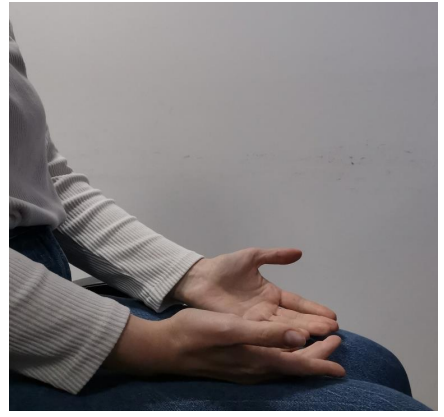
\includegraphics[scale=0.5]{exercise0}
\par\end{centering}
\caption{Resting Tremor Observation\protect\label{fig:exercise0}}

\end{figure}
\begin{figure}[H]
\begin{centering}
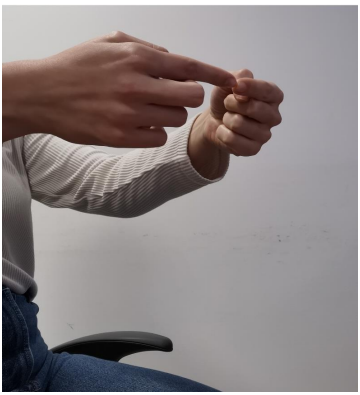
\includegraphics[scale=0.5]{exercise1}
\par\end{centering}
\caption{Test for Postural Tremor and Coordination\protect\label{fig:exercise1}}

\end{figure}
\begin{figure}[H]
\begin{centering}
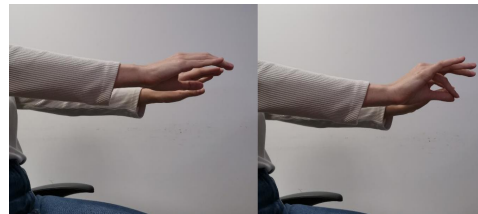
\includegraphics[scale=0.5]{exercise2}
\par\end{centering}
\caption{Finger Tapping Speed Test\protect\label{fig:exercise2}}

\end{figure}
\begin{figure}[H]
\begin{centering}
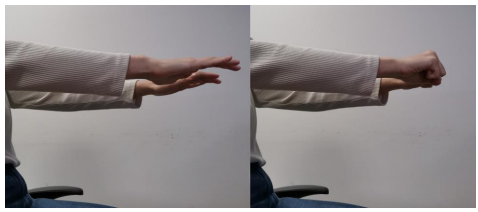
\includegraphics[scale=0.5]{exercise3}
\par\end{centering}
\caption{Hand Opening-Closing Test\protect\label{fig:exercise3}}

\end{figure}


\subsection{Feature extraction}

Numerous features were taken from the raw sensor data (accelerometer,
gyroscope, magnetometer) for each exercise in order to quantitatively
describe the motor symptoms of Parkinson's disease. These features
were computed using 50\% overlap (50 samples, 0.5 seconds) and sliding
windows of 100 samples (1 second). These features extracted are as
follows:
\begin{itemize}
\item Statistical Properties: These characteristics provide a succinct explanation
of the signal's variation and distribution. The following properties
were calculated: Skewness, Kurtosis, Quartile Deviation, Mean, Standard
Deviation, Variance, Minimum, Maximum, Range, Median, and Interquartile
Range (IQR).
\item Energy Characteristics: These metrics assess the signal's intensity
and degree of activity. Signal Magnitude Area (SMA), Root Mean Square
(RMS), Total Energy, and Logarithmic Energy are among the features
that were extracted. 
\item Frequency-Domain Features: These are essential for detecting tremors
and take into account the signal's spectral characteristics. Included
are the following features: Dominant Frequency, Spectral Flatness,
Spectral Flux, Spectral Variability, Spectral Entropy, Spectral Centroid,
Spectral Spread, and Spectral Roll-on(85\%).
\item Dynamic and Nonlinear Features: These characteristics specify the
signal's temporal fluctuations, complexity, and predictability. The
following characteristics are taken into consideration: Mean Absolute
Deviation (MAD), Root Mean Square of Successive Differences (RMSSD),
Higuchi Fractal Dimension, Lyapunov Exponent, and Sample Entropy.
\end{itemize}
Since each feature includes specific aspects of motor impairment typical
of the disease, such as tremor regularity, movement amplitude, and
signal complexity, the selection of features was driven by a large
body of literature on PD analysis. The characteristics for Movement
Analysis in Parkinson's Disease are outlined in Table \ref{tab:Table-of-Characteristics}.

\begin{table}[H]
\caption{Table of Characteristics for Movement Analysis in Parkinson's Disease.\protect\label{tab:Table-of-Characteristics}}

\raggedright{}{\scriptsize{}%
\begin{tabular}{|c|c|c|c|}
\hline 
{\scriptsize\textbf{Category}} & {\scriptsize\textbf{Characteristics}} & {\scriptsize\textbf{Purpose}} & {\scriptsize\textbf{Clinical Significance}}\tabularnewline
\hline 
\hline 
{\scriptsize Central Tendency} & {\scriptsize Mean, Median} & \begin{cellvarwidth}[t]
\centering
{\scriptsize Median Measures the central value }\\
{\scriptsize of the signal}
\end{cellvarwidth} & \begin{cellvarwidth}[t]
\centering
{\scriptsize Detection of bradykinesia }\\
{\scriptsize (slowed movements)}
\end{cellvarwidth}\tabularnewline
\hline 
{\scriptsize Dispersion} & \begin{cellvarwidth}[t]
\centering
{\scriptsize Standard deviation, }\\
{\scriptsize Variance, IQR, QD}
\end{cellvarwidth} & {\scriptsize Quantifies the spread of data} & \begin{cellvarwidth}[t]
\centering
{\scriptsize Identifies motion variability }\\
{\scriptsize (e.g. gravity, tremor)}
\end{cellvarwidth}\tabularnewline
\hline 
{\scriptsize Range} & \begin{cellvarwidth}[t]
\centering
{\scriptsize Minimum/Maximum value,}\\
{\scriptsize{} Range}
\end{cellvarwidth} & \begin{cellvarwidth}[t]
\centering
{\scriptsize Records extreme}\\
{\scriptsize{} values}
\end{cellvarwidth} & \begin{cellvarwidth}[t]
\centering
{\scriptsize Assessment of range }\\
{\scriptsize of motion reduction}\\
{\scriptsize{} in patients with Parkinson's disease}
\end{cellvarwidth}\tabularnewline
\hline 
{\scriptsize Distribution Shape} & {\scriptsize Skewness, Kurtosis} & \begin{cellvarwidth}[t]
\centering
{\scriptsize Describes asymmetry/peakedness}\\
{\scriptsize{} of distribution}
\end{cellvarwidth} & \begin{cellvarwidth}[t]
\centering
{\scriptsize Correlation with irregular }\\
{\scriptsize motor patterns}
\end{cellvarwidth}\tabularnewline
\hline 
{\scriptsize Variability} & \begin{cellvarwidth}[t]
\centering
{\scriptsize Coefficient of Variation}\\
{\scriptsize{} (CV), MAD, RMSSD}
\end{cellvarwidth} & \begin{cellvarwidth}[t]
\centering
{\scriptsize Normalized measures }\\
{\scriptsize of dispersion}
\end{cellvarwidth} & \begin{cellvarwidth}[t]
\centering
{\scriptsize Variability differentiation before}\\
{\scriptsize{} after the treatment}
\end{cellvarwidth}\tabularnewline
\hline 
{\scriptsize Energy} & \begin{cellvarwidth}[t]
\centering
{\scriptsize Total energy, }\\
{\scriptsize Absolute Energy, RMS}
\end{cellvarwidth} & \begin{cellvarwidth}[t]
\centering
{\scriptsize Measures signal }\\
{\scriptsize intensity}
\end{cellvarwidth} & \begin{cellvarwidth}[t]
\centering
{\scriptsize Correlation with hypokinesia }\\
{\scriptsize (reduced motor energy)}
\end{cellvarwidth}\tabularnewline
\hline 
{\scriptsize Logarithmic Energy} & {\scriptsize Log Energy} & \begin{cellvarwidth}[t]
\centering
{\scriptsize Enhances subtle }\\
{\scriptsize energy changes}
\end{cellvarwidth} & {\scriptsize Detection of small changes}\tabularnewline
\hline 
{\scriptsize Spectral} & {\scriptsize Spectral Entropy, Centroid} & \begin{cellvarwidth}[t]
\centering
{\scriptsize Analyzes frequency}\\
{\scriptsize{} distribution}
\end{cellvarwidth} & \begin{cellvarwidth}[t]
\centering
{\scriptsize Localization of tremor and }\\
{\scriptsize rhythmic abnormality}
\end{cellvarwidth}\tabularnewline
\hline 
{\scriptsize Roll-off} & {\scriptsize 85\% Roll-off} & \begin{cellvarwidth}[t]
\centering
{\scriptsize Frequency band where }\\
{\scriptsize 85\% of the power is concentrated}
\end{cellvarwidth} & \begin{cellvarwidth}[t]
\centering
{\scriptsize Characterization of }\\
{\scriptsize tremor bandwidth}
\end{cellvarwidth}\tabularnewline
\hline 
{\scriptsize Dominant Frequency} & {\scriptsize Dominant Frequency} & \begin{cellvarwidth}[t]
\centering
{\scriptsize Identification of peak}\\
{\scriptsize{} frequency}
\end{cellvarwidth} & \begin{cellvarwidth}[t]
\centering
{\scriptsize Detection of Parkinson's }\\
{\scriptsize tremor (4-6Hz)}
\end{cellvarwidth}\tabularnewline
\hline 
{\scriptsize Spectral Shape} & \begin{cellvarwidth}[t]
\centering
{\scriptsize Flatness, Flux,}\\
{\scriptsize{} Variability, Dispersion}
\end{cellvarwidth} & \begin{cellvarwidth}[t]
\centering
{\scriptsize Quantifies the stability }\\
{\scriptsize of the spectrum}
\end{cellvarwidth} & \begin{cellvarwidth}[t]
\centering
{\scriptsize Unstable tremors vs. }\\
{\scriptsize rhythmic movements}
\end{cellvarwidth}\tabularnewline
\hline 
{\scriptsize Dynamics} & \begin{cellvarwidth}[t]
\centering
{\scriptsize Lyapunov Exponent, }\\
{\scriptsize Sampling Entropy}
\end{cellvarwidth} & \begin{cellvarwidth}[t]
\centering
{\scriptsize Evaluates the chaos/regularity }\\
{\scriptsize of the system}
\end{cellvarwidth} & \begin{cellvarwidth}[t]
\centering
{\scriptsize Degeneration of motor control }\\
{\scriptsize in Parkinson's}
\end{cellvarwidth}\tabularnewline
\hline 
{\scriptsize Fractal} & {\scriptsize Dimension Higuchi} & \begin{cellvarwidth}[t]
\centering
{\scriptsize Measures the complexity }\\
{\scriptsize of the signal}
\end{cellvarwidth} & \begin{cellvarwidth}[t]
\centering
{\scriptsize Loss of fine }\\
{\scriptsize motor control}
\end{cellvarwidth}\tabularnewline
\hline 
\end{tabular}}{\scriptsize\par}
\end{table}
For the tri-axial accelerometer, gyroscope, and magnetometer data,
the magnitude of the signal vector was first calculated for each time
point as 
\begin{equation}
d=\sqrt{x^{2}+y^{2}+z^{2}}\label{eq:distance}
\end{equation}
and the subsequent features were then extracted from this combined
magnitude signal to produce a single value per feature. The flowchart
of Figure illustrating the multi-domain feature extraction process
from raw sensor data, including statistical, energy, frequency-domain,
and dynamic/nonlinear features.

\begin{figure}[H]
\begin{centering}
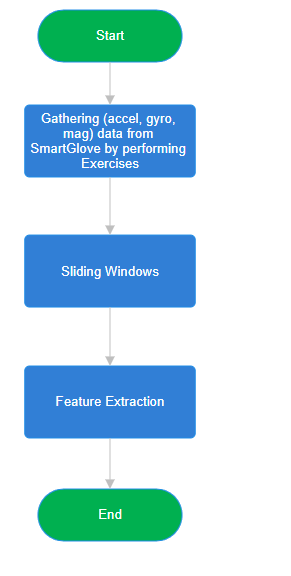
\includegraphics[scale=0.5]{flow1}
\par\end{centering}
\caption{The flowchart of he multi-domain feature extraction process from raw
sensor data.\protect\label{fig:flowExtraction}}

\end{figure}


\subsection{Feature Selection Methodology}

Feature selection is a critical step in developing accurate and interpretable
machine learning (ML) models for Parkinson’s disease (PD) detection.
In this study, a multi-method scoring approach was applied to identify
the most informative features that differentiate between pre-medication
and post-medication states. Instead of relying on a single method,
three complementary techniques were employed, and their outputs were
combined into a composite score.

\subsubsection{Multi-Method Scoring Approach}

To accurately evaluate the value of each characteristic for differentiating
between pre- and post-medication states, a multi-angled scoring approach
was adopted. For each feature, scores for three different aspects,
such as statistical significance, importance based on the model, and
variance contribution, were computed.
\begin{itemize}
\item Statistical Significance (Paired T-Test): The paired T-Test was then
carried out on measurements preceding and succeeding medication on
each dimension. To make the significance a number, the $p_{\mbox{value}}$
was transformed into a score using the following formula:
\begin{equation}
\mbox{score}_{T_{\mbox{test}}}=-\log_{10}\left(p_{\mbox{value}}+\epsilon\right)\label{eq:ttest}
\end{equation}
Here, $e=1\times10^{-10}$ is a very small constant introduced for
avoiding numerical instability arising from a $p_{\mbox{value}}$
of zero. This mapping makes variables with lower $p_{\mbox{value}}$
have exponentially large scores, hence indicating more considerable
statistical evidence against the null hypothesis ( \citep{ttest}.
\item \textbf{Model-Based Importance} (\textbf{Random Fores}t):\textbf{
}The Random Forest classifier was built such that it could distinguish
between the two different states. The importance of a specific feature
was computed using the average reduction in Gini impurity across all
trees in the ensemble. Gini impurity is a measure of the purity of
a node, and the importance is given by the weighted cumulative reduction
in node impurity, divided by the probability of the node, and averaged
across trees \citep{patel}. The calculation was performed as follows:
For a single tree $T$, the importance of feature $f$ is the sum
of its Gini impurity decreases across all nodes where it is used for
splitting: 
\begin{equation}
\mbox{Importance}_{T}\left(f\right)=\sum_{n\in S\left(T,f\right)}\Delta\mbox{Gini}\left(n,f\right)\label{eq:importance}
\end{equation}
Where $S\left(T,f\right)$ is the set of all nodes in tree $T$ split
by feature $f$, and $\Delta\mbox{Gini}\left(n,f\right)$ is the decrease
in Gini impurity at node $n$ achieved by splitting on $f$. The importance
is then averaged across all $N_{\mbox{trees}}$ trees in the forest
to obtain the final score:
\begin{equation}
\mbox{score}_{RF}(f)=\frac{1}{N_{\mbox{trees}}}\sum_{T=1}^{N_{\mbox{trees}}}\mbox{Importance}_{T}(f)\label{eq:rf}
\end{equation}
Features with a higher $\mbox{score}$$\mbox{score}_{RF}(f)$ are
more influential in the model's decision-making process.
\item \textbf{Variance Contribution} \textbf{Score }(\textbf{PCA}): Principal
Component Analysis (PCA) was performed on the standardized data set.
The contribution of a individual original feature towards the principal
components (PCs) was measured by adding its absolute loadings across
all PCs. The loading of a feature onto a PC is its correlation with
the specific component \citep{Guyon}. The score $\mbox{score}_{\mbox{PCA}}$
was computed as follows:
\begin{equation}
\mbox{score}_{\mbox{PCA}}=\sum_{i}\left|\mbox{loading}_{i}\right|\label{eq:pca}
\end{equation}
Here, the $\mbox{loading}_{i}$ is the feature weight corresponding
to the $i$-th principal component. This cumulative sum provides the
total impact of the feature on the total variance tackled by the Principal
Component Analysis (PCA) model \citep{pcaReview}.
\end{itemize}

\subsubsection{Composite Score Calculation}

To reduce these unrelated measurements into one unified measure of
feature prominence, the scores were amalgamated. Each score was first
normalized between $[0,1]$ using min-max normalization for comparability
across scores. A clear composite score was then calculated as a weighted
average of the normalized scores: 
\begin{equation}
\mbox{Composite Score}=\mbox{0.4\ensuremath{\times}score}_{T_{\mbox{test}}}+0.3\times\mbox{score}_{RF}+0.3\times\mbox{score}_{\mbox{PCA}}\label{eq:composite}
\end{equation}
This weighting approach was chosen so that features which are highly
statistically significant (by the T-test) are given priority, first,
while data from model-based learning (Random Forest) and variance-based
analysis (PCA) are incorporated cautiously

\subsubsection{Selection of best features}

Features were ranked according to their composite score, and the top-performing
ones were selected for subsequent model development. Representative
high-ranking features includes:
\begin{itemize}
\item RMSSD from the gyroscope during Exercise 2 (score: 0.663),
\item Lyapunov Exponent (score: 0.644),
\item Higuchi Fractal Dimension (score: 0.612).
\end{itemize}
These selected features served as the foundation for later predictive
modeling and analysis, aiming to capture the most relevant motor signal
characteristics associated with PD symptoms \citep{goetz,chen}. In
Table \ref{tab:Top-20-features} the top 20 features are presented.

\begin{table}[H]
\caption{Top 20 features scored\protect\label{tab:Top-20-features}}

\centering{}%
\begin{tabular}{|c|c|c|c|}
\hline 
Exercise & Sensor & \begin{cellvarwidth}[t]
\centering
Feature \\
Name
\end{cellvarwidth} & \begin{cellvarwidth}[t]
\centering
Composite\\
Score
\end{cellvarwidth}\tabularnewline
\hline 
\hline 
2 & gyro & rmssd & 0.663\tabularnewline
\hline 
2 & gyro & lyapunov\_exponent & 0.644\tabularnewline
\hline 
2 & gyro & higuchi\_fractal\_dimension & 0.612\tabularnewline
\hline 
2 & gyro & range & 0.573\tabularnewline
\hline 
3 & acce & higuchi\_fractal\_dimension & 0.469\tabularnewline
\hline 
3 & gyro & max & 0.452\tabularnewline
\hline 
3 & acce & lyapunov\_exponent & 0.437\tabularnewline
\hline 
2 & gyro & spectral\_rolloff & 0.433\tabularnewline
\hline 
2 & acce & sample\_entropy & 0.422\tabularnewline
\hline 
0 & magn & lyapunov\_exponent & 0.406\tabularnewline
\hline 
0 & magn & spectral\_variability & 0.399\tabularnewline
\hline 
0 & magn & higuchi\_fractal\_dimension & 0.399\tabularnewline
\hline 
0 & magn & range & 0.381\tabularnewline
\hline 
3 & magn & rmssd & 0.376\tabularnewline
\hline 
0 & gyro & rmssd & 0.375\tabularnewline
\hline 
2 & gyro & std & 0.373\tabularnewline
\hline 
3 & acce & spectral\_flux & 0.367\tabularnewline
\hline 
1 & gyro & lyapunov\_exponent & 0.365\tabularnewline
\hline 
1 & gyro & rmssd & 0.361\tabularnewline
\hline 
1 & gyro & max & 0.358\tabularnewline
\hline 
\end{tabular}
\end{table}
Following the ranking by composite score, the top 80\% of features
were retained for the subsequent model development and feature construction
process.

\subsection{Grammatical Evolution preliminaries \protect\label{subsec:Preliminaries}}

Grammatical Evolution procedure can be considered as a genetic algorithm,
where the chromosomes are sets of randomly chosen integers. These
integers represent production rules of the provided BNF grammar \citep{bnf1}.
BNF grammars are usually expressed as sets having the form \textbf{$G=\left(N,T,S,P\right)$},
where
\begin{itemize}
\item The set\textbf{ $N$ }contains the non-terminal symbols of the grammar.
\item The set \textbf{$T$ }includes the terminal symbols of the grammar.\textbf{ }
\item $S$ denotes the start symbol of the grammar, with $S\in N$.
\item \textbf{$P$ }is the set of production rules of the grammar. 
\end{itemize}
The Grammatical Evolution procedure utilizes an extended version of
the initial BNF grammar by adding enumeration in the the production
rules. As an example of an extended BNF grammar consider the grammar
shown in\textbf{ }Figure \ref{fig:BNF-grammar-of}.\textbf{ }The notation
\textless{} \textgreater{} is used to enclose the non - terminal symbols
of the grammar. The value $d$ denotes the dimension of the input
data. The Grammatical Evolution procedure starts from the start symbol
of the program and gradually it creates valid programs in the underlying
language, using the production rules of the grammar. The general scheme
of the production procedure has as follows:
\begin{itemize}
\item \textbf{Get} the next element V from the chromosome that is under
processing.
\item \textbf{Select} the next rule using the equation Rule = V mod NR.
The symbol NR denotes the number of production rules for the under
processing non -- terminal symbol. 
\end{itemize}
A full working example of the production procedure is the chromosome
\[
x=\left[9,8,6,4,16,10,17,23,8,14\right]
\]
 with $d=3$. After a series of steps, the function $f(x)=x_{2}+\cos\left(x_{3}\right)$
is produced for the grammar of Figure \ref{fig:BNF-grammar-of}. The
production steps are shown in Table \ref{tab:table_with_steps}. 

\begin{figure}[H]
\caption{An example of an extended BNF grammar.\protect\label{fig:BNF-grammar-of}}

\begin{lyxcode}
S::=\textless expr\textgreater ~~~(0)~

\textless expr\textgreater ~::=~~(\textless expr\textgreater ~\textless op\textgreater ~\textless expr\textgreater )~~(0)~~~~~~~~~~~~~

~~~~~~~~~~~\textbar ~\textless func\textgreater ~(~\textless expr\textgreater ~)~~~~(1)~~~~~~~~~~~~~

~~~~~~~~~~~\textbar\textless terminal\textgreater ~~~~~~~~~~~~(2)~

\textless op\textgreater ~::=~~~~~+~~~~~~(0)~~~~~~~~~~~~~

~~~~~~~~~~~\textbar ~-~~~~~~(1)~~~~~~~~~~~~~

~~~~~~~~~~~\textbar ~{*}~~~~~~(2)~~~~~~~~~~~~~

~~~~~~~~~~~\textbar ~/~~~~~~(3)

\textless func\textgreater ~::=~~~sin~~(0)~~~~~~~~~~~~~

~~~~~~~~~~~\textbar ~cos~~(1)~~~~~~~~~~~~~

~~~~~~~~~~~\textbar exp~~~(2)~~~~~~~~~~~~~

~~~~~~~~~~~\textbar log~~~(3)

\textless terminal\textgreater ::=\textless xlist\textgreater ~~~~~~~~~~~~~~~~(0)~~~~~~~~~~~~~~~~~~~~~~

~~~~~~~~~~~\textbar\textless dlist\textgreater .\textless dlist\textgreater ~(1)

\textless xlist\textgreater ::=x1~~~~(0)~~~~~~~~~~~~~~

~~~~~~~~~~~\textbar ~x2~(1)~~~~~~~~~~~~~~

~~~~~~~~~~~………~~~~~~~~~~~~~

~~~~~~~~~~~\textbar ~xd~(d-1)

\textless dlist\textgreater ::=\textless digit\textgreater ~~~~~~~~~~~~~~~~~~(0)~~~~~~~~~~~~~~~~~

~~~~~~~~~~~\textbar ~\textless digit\textgreater\textless digit\textgreater ~~~~~~~~~~~~(1)

~~~~~~~~~~~\textbar ~\textless digit\textgreater\textless digit\textgreater\textless digit\textgreater ~~~~~(2)

\textless digit\textgreater ~~::=~0~(0)~~~~~~~~~~~~~

~~~~~~~~~~~\textbar ~1~(1)~~~~~~~~~~~~~

~~~~~~~~~~~\textbar ~2~(2)~~~~~~~~~~~~~

~~~~~~~~~~~\textbar ~3~(3)~~~~~~~~~~~~~

~~~~~~~~~~~\textbar ~4~(4)~~~~~~~~~~~~~

~~~~~~~~~~~\textbar ~5~(5)~~~~~~~~~~~~~

~~~~~~~~~~~\textbar ~6~(6)~~~~~~~~~~~~~

~~~~~~~~~~~\textbar ~7~(7)~~~~~~~~~~~~~

~~~~~~~~~~~\textbar ~8~(8)~~~~~~~~~~~~~

~~~~~~~~~~~\textbar ~9~(9)
\end{lyxcode}
\end{figure}
\begin{table}[H]
\caption{A series of production steps for the example chromosome. \protect\label{tab:table_with_steps}}

\centering{}%
\begin{tabular}{|c|c|c|}
\hline 
String & Chromosome & Operation\tabularnewline
\hline 
\hline 
\textless expr\textgreater{} & 9,8,6,4,16,10,17,23,8,14 & $9\mod 3=0$\tabularnewline
\hline 
(\textless expr\textgreater\textless op\textgreater\textless expr\textgreater ) & 8,6,4,16,10,17,23,8,14 & $8\mod 3=2$\tabularnewline
\hline 
(\textless terminal\textgreater\textless op\textgreater\textless expr\textgreater ) & 6,4,16,10,17,23,8,14 & $6\mod 2=0$\tabularnewline
\hline 
(\textless xlist\textgreater\textless op\textgreater\textless expr\textgreater ) & 4,16,10,17,23,8,14 & $4\mod 3=1$\tabularnewline
\hline 
(x2\textless op\textgreater\textless expr\textgreater ) & 16,10,17,23,8,14 & $16\mod 4=0$\tabularnewline
\hline 
(x2+\textless expr\textgreater ) & 10,17,23,8,14 & $10\mod 3=1$\tabularnewline
\hline 
(x2+\textless func\textgreater (\textless expr\textgreater )) & 17,23,8,14 & $17\mod 4=1$\tabularnewline
\hline 
(x2+cos(\textless expr\textgreater )) & 23,8,14 & $23\mod 2=2$\tabularnewline
\hline 
(x2+cos(\textless terminal\textgreater )) & 8,14 & $8\mod 2=0$\tabularnewline
\hline 
(x2+cos(\textless xlist\textgreater )) & 14 & $14\mod 3=2$\tabularnewline
\hline 
(x2+cos(x3)) &  & \tabularnewline
\hline 
\end{tabular}
\end{table}


\subsection{The feature construction method\protect\label{subsec:The-feature-construction}}

The technique of feature construction produces artificial features
for classification or regression problems as non - linear transformations
of the original ones. The new features are evaluated using a machine
learning technique, such as artificial neural networks \citep{nn1,nn2}
or a Radial Basis Function (RBF) networks \citep{rbf1,rbf2}. This
method was presented initially in \citep{fc1}. Also, this method
was used in many areas, such as Spam Identification \citep{fc2},
Fetal heart classification \citep{fc3},\textbf{ }signal processing
\citep{fc4,fc5} etc. The process has the following steps:
\begin{enumerate}
\item \textbf{Initialization} step. \textbf{}

\begin{enumerate}
\item \textbf{Obtain }the train data for the current problem. The train
data have $M$ pairs\textbf{ $\left(x_{i},t_{i}\right),\ i=1..M$}.
The dimension of each vector $x_{i}$ is\textbf{ $d$.} The values
$t_{i}$ are the expected outputs for each pattern.
\item \textbf{Define }the parameters of the genetic algorithm: \textbf{$N_{g}$}
stands for the the number of allowed generations, \textbf{$N_{c}$
}represents the number chromosomes,\textbf{ $p_{s}$ }defines the
selection rate and \textbf{$p_{m}$} the mutation rate.
\item \textbf{Set} as $N_{f}$ the number of features that will construct
the Grammatical Evolution procedure.
\item \textbf{Initialize} the chromosomes in the population. Each chromosome
is considered as a set of randomly chosen positive integers.
\item \textbf{Set} $k=1$, as the generation counter.
\end{enumerate}
\item \textbf{Genetic step}

\begin{enumerate}
\item \textbf{For $i=1,\ldots,N_{c}$ do}

\begin{enumerate}
\item \textbf{Produce} using the Grammatical Evolution procedure a set of
$N_{f}$ artificial features for the corresponding chromosome $g_{i}$.
These features are produced using the grammar of Figure \ref{fig:BNF-grammar-of}.
\item \textbf{Transform} the original dataset using the previously constructed
features. The new training set is denoted as $\left(x_{g_{i},j},t_{j}\right),\ j=1,..M$
\item \textbf{Train }a machine learning model denoted as $C$ using the
new training set. The fitness $f_{i}$ for the corresponding chromosome
is defined as:
\begin{equation}
f_{i}=\sum_{j=1}^{M}\left(C\left(x_{g_{i},j}\right)-t_{j}\right)^{2}
\end{equation}
In the proposed method the RBF network is used as the machine learning
model, since the time required for its training is significantly lower
than other models, such as neural networks.
\item \textbf{Perform} the selection procedure. During this procedure the
chromosomes are firstly sorted according to their fitness values and
the best\textbf{ $\left(1-p_{s}\right)\times N_{C}$} of them are
copied intact to the next generation.\textbf{ }The rest of the chromosomes
will be substituted by new chromosomes produced during the procedures
of crossover and mutation. 
\item \textbf{Perform} the crossover procedure. During this procedure $p_{s}\times N_{c}$
new chromosomes are produced. For every pair of $\left(\tilde{z},\tilde{w}\right)$
of new chromosomes, two two distinct chromosomes $\left(z,w\right)$
are selected from the current population. The selection is performed
using the tournament selection. The new chromosomes are produced from
the old ones using the one - point crossover procedure, which is graphically
outlined in Figure \ref{fig:One-point-crossover}. 
\item \textbf{Perform} the mutation procedure: for each each element of
each chromosome, a random number $r\in\left[0,1\right]$ is selected.
The underlying element is altered randomly when $r\le p_{m}$. 
\end{enumerate}
\item \textbf{EndFor}
\end{enumerate}
\item \textbf{Set} $k=k+1$
\item \textbf{If} $k\le N_{G}$ goto \textbf{Genetic} Step, else terminate
the process and obtain the best chromosome $g^{*}$ with the lowest
fitness value.
\item \textbf{Transform} the corresponding test set, using the $N_{f}$
features obtained for chromosome \textbf{$g^{*}$.}
\item \textbf{Apply} a machine learning model to the constructed test set
and report the associated test error.\textbf{.}

\end{enumerate}
\begin{figure}[H]
\begin{centering}
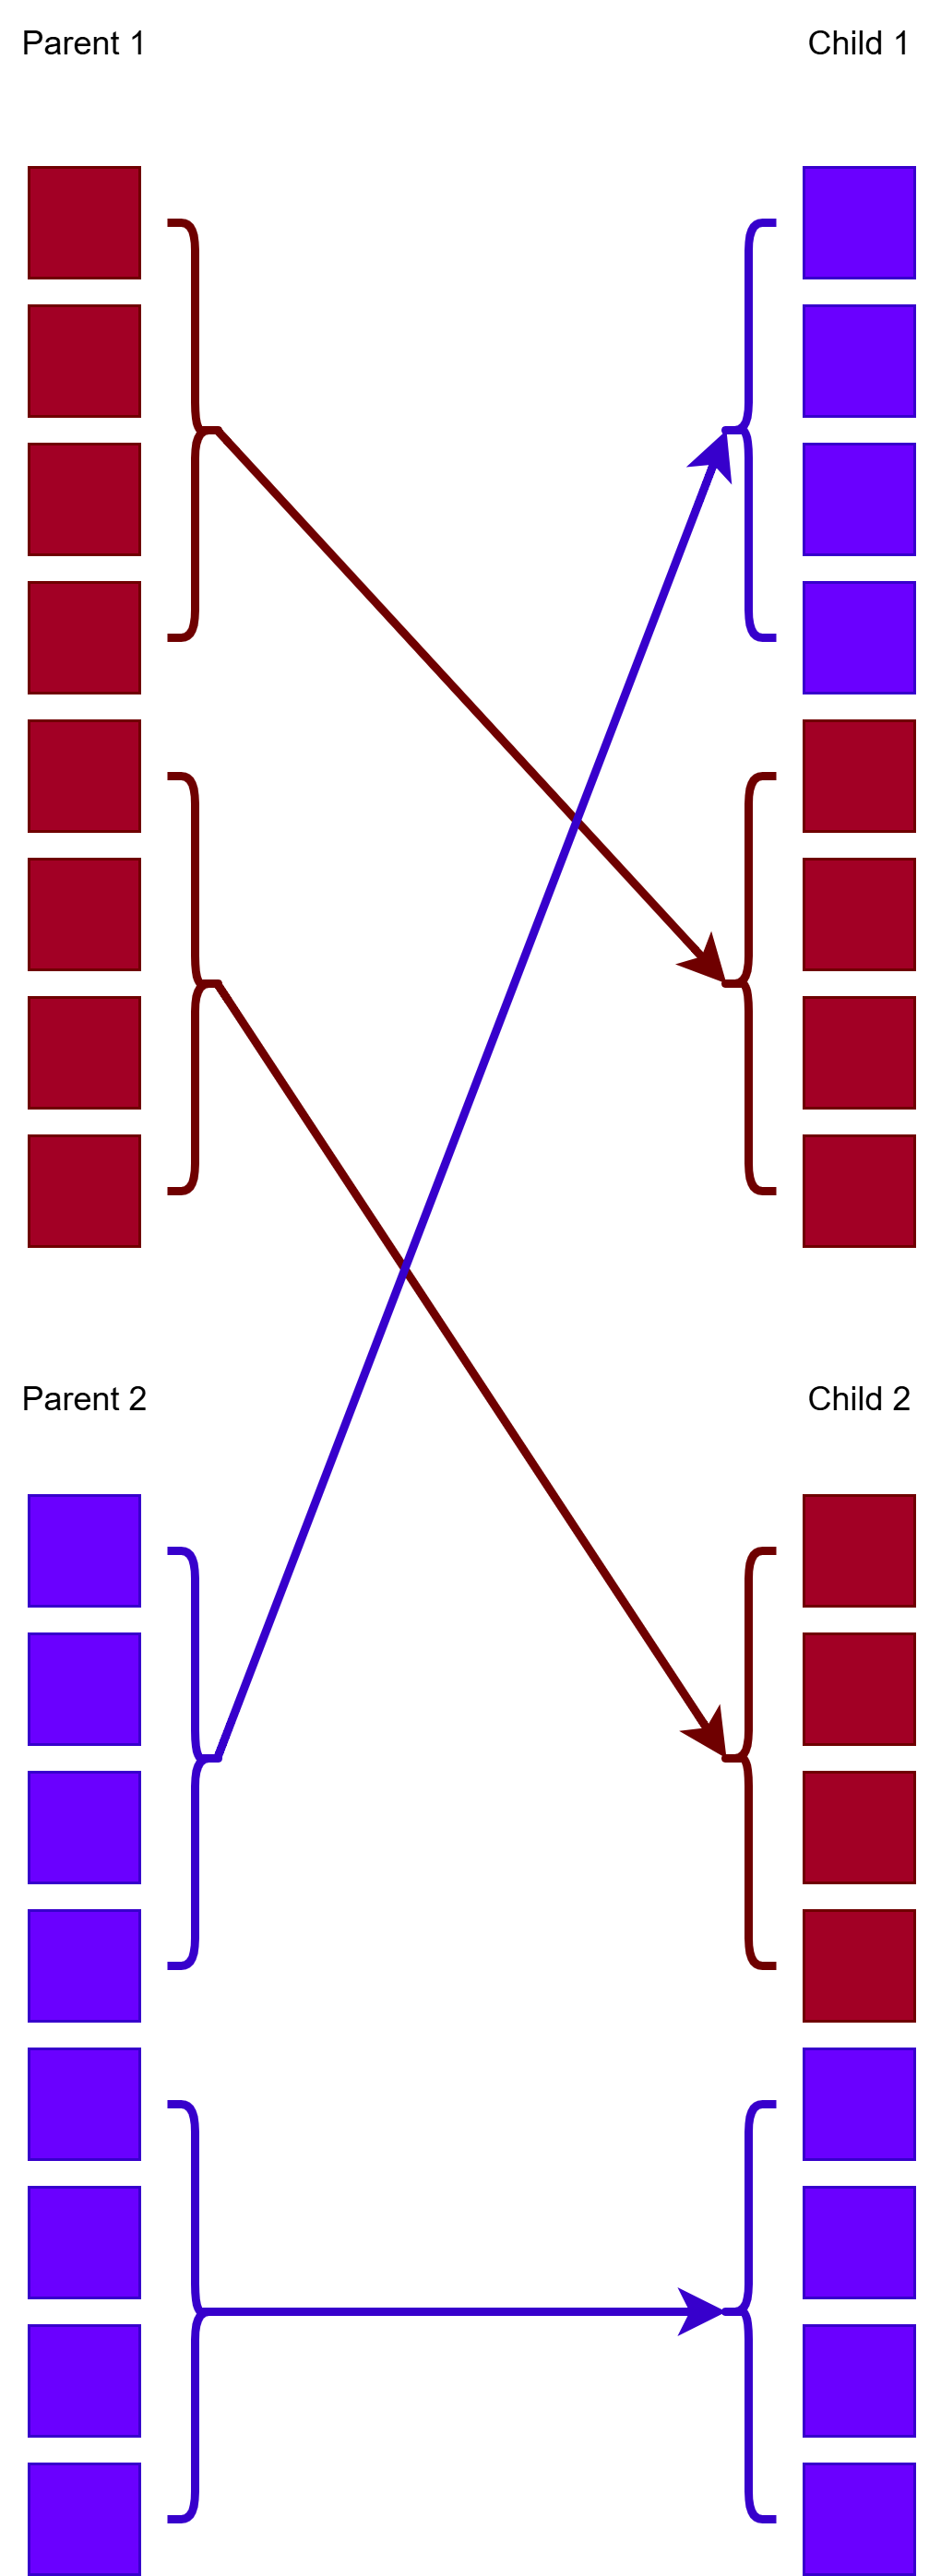
\includegraphics[scale=0.5]{cross2}
\par\end{centering}
\caption{One point crossover method, used in the Grammatical Evolution procedure.\protect\label{fig:One-point-crossover}}
\end{figure}
A flowchart of the previous algorithm is shown in Figure \ref{fig:Flowchart-of-the}.

\begin{figure}[H]
\begin{centering}
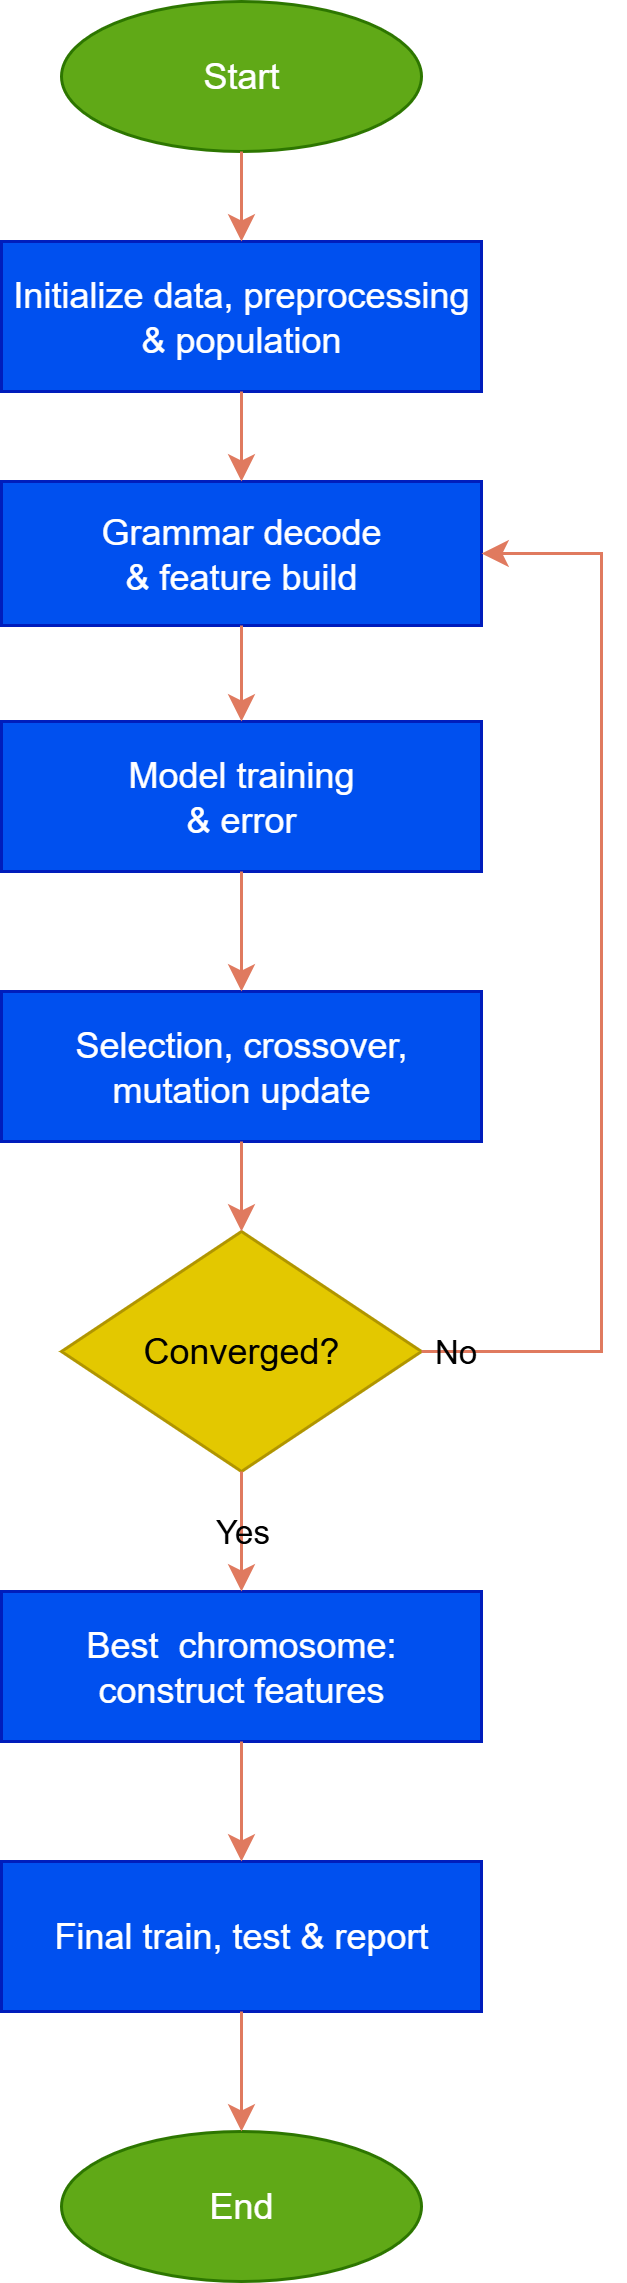
\includegraphics[scale=0.5]{flow}
\par\end{centering}
\caption{Flowchart of the used genetic algorithm.\protect\label{fig:Flowchart-of-the}}

\end{figure}
 The flowchart that describes the proposed methodology for Parkinson’s
Disease motor symptom analysis, from data acquisition using the SmartGlove
to feature construction and classification is shown in Figure \ref{fig:End-to-end-flowchart-of}.

\begin{figure}[H]
\begin{centering}
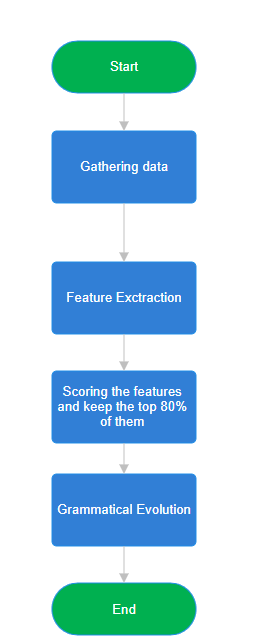
\includegraphics[scale=0.5]{flowWhole}
\par\end{centering}
\caption{End-to-end flowchart of the proposed methodology for Parkinson’s Disease
motor symptom analysis, from data acquisition using the SmartGlove
to feature construction and classification.\protect\label{fig:End-to-end-flowchart-of}}

\end{figure}


\section{Results\protect\label{sec:Results}}

The code used in the experiments was code in the C++ programming language
and for the optimization methods the freely available Optimus programming
tool was incorporated \citep{optimus}. The experiments were conducted
on machine with 128GB of ram, running the Debian Linux operating system.
Each experiment was executed 30 times and the average classification
error was measured and depicted in the related tables and graphs.
Also, the 10 - fold cross validation technique was incorporated for
the validation of the experimental results. The values for the parameters
of the proposed method are depicted in Table  \ref{tab:settings}.\textbf{
}
\begin{table}[H]
\caption{The values for the parameters for the current work.\protect\label{tab:settings}}

\centering{}%
\begin{tabular}{|c|c|c|}
\hline 
PARAMETER & MEANING & VALUE\tabularnewline
\hline 
\hline 
$N_{g}$ & Number of maximum allowed generations. & 500\tabularnewline
\hline 
$N_{c}$ & Number of chromosomes & 500\tabularnewline
\hline 
$p_{s}$ & Selection rate & 0.10\tabularnewline
\hline 
$p_{m}$ & Mutation rate & 0.05\tabularnewline
\hline 
$H$ & Number of processing nodes for neural network & 10\tabularnewline
\hline 
\end{tabular}
\end{table}
\textbf{ }

In the experimental tables the following notation is used:
\begin{enumerate}
\item The column DATASET represents the performed exercise.
\item The column RBF stands for the application of an RBF neural network
\citep{rbf1,rbf2} with 10 processing nodes on the corresponding dataset.
\item The column GEN represents the application of a genetic algorithm \citep{geneticnn}
on the training process of a neural network with 10 processing nodes.
\item The column PCA stands for the application of the PCA method \citep{nnpca1,nnpca2,nnpca3}
to construct two artificial features from the original ones. Afterwards,
a neural network with 10 processing nodes trained using the BFGS method
is applied on the new datasets.
\item The column NNC stands for the application of a neural network constructed
with Grammatical Evolution \citep{nnc} on the corresponding dataset.
\item The column GENCLASS represents the usage of a method that constructs
classification rules using Grammatical Evolution \citep{genclass}.
\item The column FC2 is used to represent the application of a genetic algorithm
to train a neural network on the dataset produced by the construction
of two artificial features using the feature construction method.
\item The column FC3 is used to represent the application of a genetic algorithm
to train a neural network on the dataset produced by the construction
of three artificial features using the feature construction method.
\item The column FC4 is used to represent the application of a genetic algorithm
to train a neural network on the dataset produced by the construction
of four artificial features using the feature construction method.
\item The row AVERAGE represents the average classification error for all
datasets and the corresponding method.
\end{enumerate}
Table \ref{tab:exper} reports classification error per exercise and
per feature/model family, where lower values are better. The proposed
Feature Construction approach (columns FC2, FC3 and FC4) consistently
yields lower errors than classical baselines such as PCA, RBF, NNC,
GEN and GENCLASS, indicating that the constructed descriptors capture
the discriminative motion patterns more effectively. Based on the
overall average, FC3 is the strongest among the proposed variants,
achieving the lowest mean error, with FC4 very close behind and FC2
also competitive. In EXERCISE 0 the Feature Construction variants
clearly dominate, with FC3 providing the best balance between expressiveness
and generalization, FC4 performing nearly as well, and FC2 remaining
stable. In EXERCISE 1 the picture is similar: FC2--FC4 retain a lead
over classical pipelines and FC3 acts as the “sweet spot,” while FC4
is the slightly more aggressive variant and FC2 the conservative yet
reliable option. In EXERCISE 2, where separability is more challenging,
the FC columns keep the error noticeably lower than the classical
models and FC3 generally maintains an edge, although FC4 occasionally
approaches or overlaps within small margins. In EXERCISE 3 the same
trend holds, with FC2, FC3 and FC4 achieving lower errors and FC3
preserving the overall lead among the proposed methods. Overall, Table
5 underscores that representation quality precedes classifier complexity;
when features are properly constructed, even relatively simple decision
rules can achieve consistently low error. In practice, orchestrating
Feature Construction with linear or RBF-based decision layersor adopting
a hybrid design where feature construction is followed by mild dimensionality
reduction preserves the information advantage while further controlling
noise. The average results for this table are also outlined graphically
in Figure \ref{fig:The-average-classification}.

\begin{table}[H]
\caption{Experimental results for various exercises.\protect\label{tab:exper}}

\raggedright{}{\footnotesize{}%
\begin{tabular}{|c|c|c|c|c|c|c|c|c|}
\hline 
{\footnotesize DATASET} & {\footnotesize RBF} & {\footnotesize GEN} & {\footnotesize PCA} & {\footnotesize NNC} & {\footnotesize GENCLASS} & {\footnotesize FC2} & {\footnotesize FC3} & {\footnotesize FC4}\tabularnewline
\hline 
\hline 
{\footnotesize EXERCISE 0} & {\footnotesize 40.86\%} & {\footnotesize 39.63\%} & {\footnotesize 44.70\%} & {\footnotesize 32.57\%} & {\footnotesize 25.52\%} & {\footnotesize 11.39\%} & {\footnotesize 11.06\%} & {\footnotesize 10.35\%}\tabularnewline
\hline 
{\footnotesize EXERCISE 1} & {\footnotesize 38.65\%} & {\footnotesize 47.61\%} & {\footnotesize 47.35\%} & {\footnotesize 42.07\%} & {\footnotesize 29.98\%} & {\footnotesize 20.16\%} & {\footnotesize 16.08\%} & {\footnotesize 14.84\%}\tabularnewline
\hline 
{\footnotesize EXERCISE 2} & {\footnotesize 37.57\%} & {\footnotesize 35.33\%} & {\footnotesize 40.46\%} & {\footnotesize 35.01\%} & {\footnotesize 31.34\%} & {\footnotesize 22.50\%} & {\footnotesize 19.78\%} & {\footnotesize 22.10\%}\tabularnewline
\hline 
{\footnotesize EXERCISE 3} & {\footnotesize 41.64\%} & {\footnotesize 39.17\%} & {\footnotesize 43.46\%} & {\footnotesize 35.88\%} & {\footnotesize 29.00\%} & {\footnotesize 19.79\%} & {\footnotesize 17.39\%} & {\footnotesize 19.91\%}\tabularnewline
\hline 
\end{tabular}}{\footnotesize\par}
\end{table}
\begin{figure}[H]
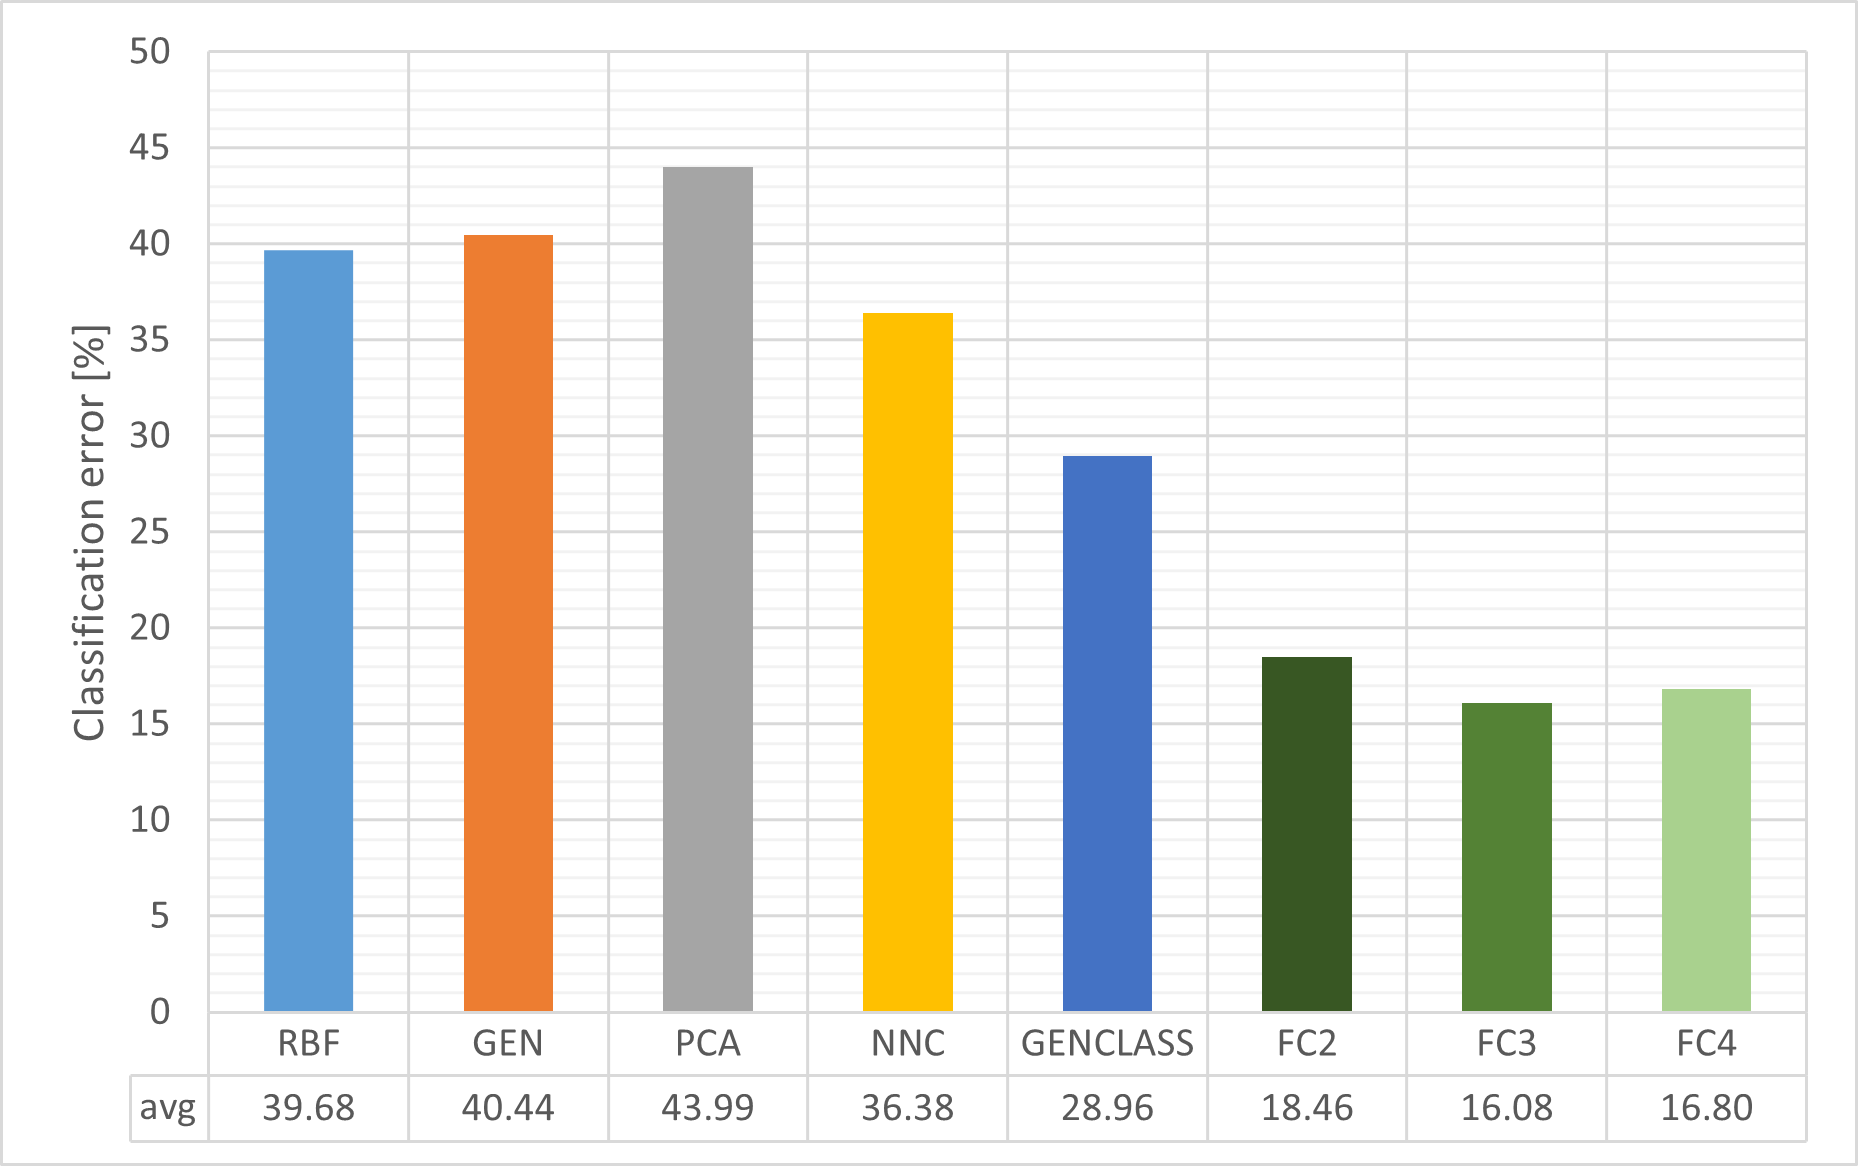
\includegraphics{parkinson_bars}

\caption{The average classification error for all methods participated in the
experiments.\protect\label{fig:The-average-classification}}

\end{figure}
Also the precision values for all exercises and machine learning methods
are outlined in Table \ref{tab:Precision-values.}. Similarly, the
recall values are depicted in Table \ref{tab:Recall-values.}.

\begin{table}[H]
\caption{Precision values for all methods participated in the experiments.\protect\label{tab:Precision-values.}}

\raggedright{}{\footnotesize{}%
\begin{tabular}{|c|c|c|c|c|c|c|c|c|}
\hline 
{\footnotesize DATASET} & {\footnotesize RBF} & {\footnotesize GEN} & {\footnotesize PCA} & {\footnotesize NNC} & {\footnotesize GENCLASS} & {\footnotesize FC2} & {\footnotesize FC3} & {\footnotesize FC4}\tabularnewline
\hline 
\hline 
{\footnotesize EXERCISE 0} & {\footnotesize 0.589} & {\footnotesize 0.603} & {\footnotesize 0.559} & {\footnotesize 0.673} & {\footnotesize 0.761} & {\footnotesize 0.885} & {\footnotesize 0.889} & {\footnotesize 0.898}\tabularnewline
\hline 
{\footnotesize EXERCISE 1} & {\footnotesize 0.62} & {\footnotesize 0.496} & {\footnotesize 0.581} & {\footnotesize 0.595} & {\footnotesize 0.713} & {\footnotesize 0.795} & {\footnotesize 0.837} & {\footnotesize 0.851}\tabularnewline
\hline 
{\footnotesize EXERCISE 2} & {\footnotesize 0.616} & {\footnotesize 0.726} & {\footnotesize 0.582} & {\footnotesize 0.646} & {\footnotesize 0.69} & {\footnotesize 0.778} & {\footnotesize 0.803} & {\footnotesize 0.78}\tabularnewline
\hline 
{\footnotesize EXERCISE 3} & {\footnotesize 0.583} & {\footnotesize 0.608} & {\footnotesize 0.566} & {\footnotesize 0.642} & {\footnotesize 0.715} & {\footnotesize 0.803} & {\footnotesize 0.829} & {\footnotesize 0.803}\tabularnewline
\hline 
\end{tabular}}{\footnotesize\par}
\end{table}
\begin{table}[H]
\caption{Recall values for all methods used in the conducted experiments.\protect\label{tab:Recall-values.}}

\raggedright{}{\footnotesize{}%
\begin{tabular}{|c|c|c|c|c|c|c|c|c|}
\hline 
{\footnotesize DATASET} & {\footnotesize RBF} & {\footnotesize GEN} & {\footnotesize PCA} & {\footnotesize NNC} & {\footnotesize GENCLASS} & {\footnotesize FC2} & {\footnotesize FC3} & {\footnotesize FC4}\tabularnewline
\hline 
\hline 
{\footnotesize EXERCISE 0} & {\footnotesize 0.588} & {\footnotesize 0.603} & {\footnotesize 0.559} & {\footnotesize 0.689} & {\footnotesize 0.75} & {\footnotesize 0.883} & {\footnotesize 0.885} & {\footnotesize 0.893}\tabularnewline
\hline 
{\footnotesize EXERCISE 1} & {\footnotesize 0.619} & {\footnotesize 0.766} & {\footnotesize 0.605} & {\footnotesize 0.626} & {\footnotesize 0.711} & {\footnotesize 0.797} & {\footnotesize 0.839} & {\footnotesize 0.854}\tabularnewline
\hline 
{\footnotesize EXERCISE 2} & {\footnotesize 0.626} & {\footnotesize 0.646} & {\footnotesize 0.589} & {\footnotesize 0.653} & {\footnotesize 0.674} & {\footnotesize 0.771} & {\footnotesize 0.801} & {\footnotesize 0.78}\tabularnewline
\hline 
{\footnotesize EXERCISE 3} & {\footnotesize 0.583} & {\footnotesize 0.608} & {\footnotesize 0.567} & {\footnotesize 0.652} & {\footnotesize 0.713} & {\footnotesize 0.801} & {\footnotesize 0.827} & {\footnotesize 0.802}\tabularnewline
\hline 
\end{tabular}}{\footnotesize\par}
\end{table}


\section{Discussion\protect\label{sec:Discussion}}

\subsection{Comparison of Motor Exercises Study}

The performance of our models was inconsistent across the four exercises,
but it also gave us important information about which motor activities
produce the most discriminative data for distinguishing pre- and post-medication
conditions. The easiest task for classification was Exercise 0 (Resting
Tremor Observation), for all FC models produced the best results with
the least error rates of around 10-11\%. The excellent performance
here implies that resting-state kinematics, almost certainly including
subtle tremor and rigidity, are greatly and reliably impacted by medication.
The relative ease of such a task ensures that, to some extent, \textquotedbl voluntary
noise\textquotedbl{} due to move decisions is minimized, such that
the model isolates essential pathological signatures that were reliably
modulated by medicine. On the other hand, Exercises 2 and 3 (Finger
Tapping and Hand Opening-Closing), as tests for bradykinesia and rigidity,
also had good results but with slightly elevated error rates. The
rapid, repeated character of these tests for generating rich dynamic
and non-linear data, and the saliency of features such as the Root
Mean Square of Successive Differences (RMSSD), and the Lyapunov Exponent
of the gyroscope, highlight that the smoothness and predictability
of motion is a chief biomarker. Finally, Exercise 1 (Postural Tremor
and Coordination) was the most difficult for our models. The complexity
of the task, with more complex planning of motor actions, can create
data with higher inter-subject variability or can involve neurobiological
circuitry that is less reliably impacted by medication in the short-term.
In conclusion, while all of these exercises contributed, the most
reliable information for the production of discriminative features
in such a specific classification task were the resting tremor observation
and specifically conducted bradykinesia tests.

\subsection{Effectiveness of the Multi-Method Feature Scoring System}

One of the key contributions of the present work is the composite
feature scoring system, whereby it was successful in finding a sparse
set of highly relevant biomarkers without prior recourse to a particular
ML algorithm. The power of such an approach is in the tripartite validation,
whereby it combined statistical significance, model-driven importance,
and variance contribution. The first, the statistical T-test, ensured
that all chosen features had a significant mean shift between pharmacological
states at the population scale, a prerequisite for a useful biomarker.
The second, the Random Forest importance, assessed each feature's
informativeness in a non-linear, ensemble learning framework, highlighting
those that were most effective in splitting the data. The third, PCA
variance contribution, ensured that chosen features captured prominent
patterns in the dataset, optimizing for non-redundancy. Empirical
verification of such a strategy is in the composition of the top-ranked
features, whereby they were dominated by non-linear dynamic measures
such as the Lyapunov exponent and Higuchi fractal dimension. This
suggests that the system successfully ranked features that described
the complexity and chaos of PD motor control as most important, something
these sorts of simplistic statistical mean-based methods oftentimes
fail to capture. The reason why these very features subsequently became
the foundation of the highly successful Grammatical Evolution process
is that it empirically identifies that the scoring system was extraordinarily
successful in reducing the raw feature space to the most physiologically
relevant candidates of biomarkers, with the direct consequence being
the dramatic reduction in classification error. Hence, this is not
so much a victory of the ultimate model, but rather a direct consequence
of such a rigorous, multi-faced scoring system that revealed these
data-driven biomarkers most relevant to the patient pharmacological
state.

\subsection{Limitations and Future Work}

Despite the successful findings, the current study is limited by specific
drawbacks that define clear paths for future research. Foremost among
these is partial activation of the full sensor complement of the SmartGlove.
While the information gathered through the inertial measurement unit
(IMU) was very informative, incremental information that potentially
could arrive through the flex sensors and finger-to-palm touch sensors
was not utilized in this evaluation. These sensors may be used to
offer direct, quantitative measures of bradykinesia and rigidity---the
range and velocity of finger flexion, for example, and the completeness
of finger-tapping contacts---in values that at present are inferred
exclusively based on IMU kinematics. The application of these sensors
in subsequent studies would allow for derivation of a more-complete
digital model of hand motor function.

Additionally, the range of this research was limited by a modestly
sized pool of participants. To legitimize the reliability and portability
of the thus derived features, a larger and more heterogeneous dataset
is required, that would encompass patients in various stages of Parkinson's
Disease, in association with various age groups, illness duration,
and treatment regimens. It would make the feature selection process
statistically more robust and legitimize that the thus determined
biomarkers would represent the whole PD population, rather than being
unique to some subgroup, only. To overcome such identified limitations
and extend our findings further, our subsequent research will follow
multiple avenues. The near-term is the full integration of data from
the flex and contact sensors into the feature extraction protocol,
thus generating a unified multi-modal dataset more comprehensively
capturing the phenomenology of hand motion. Concurrently, we initiate
a large-scale clinical validation study for the purpose of collecting
data from a much larger population of subjects in diverse clinical
settings. This project shall allow us not only to verify the efficacy
of our present features but also examine the feasibility of developing
models for patient stratification by disease severity or for the prediction
of individual responses to therapy. Our long-term aim is to develop
this methodology into a useful, sustained, at-home, practical monitor,
providing continuous, objective information for personalized therapeutic
strategies for Parkinson's Disease.

\section{Conclusions\protect\label{sec:Conclusions}}

This study successfully formulated a rigorous methodology for the
unbiased assessment of motor symptoms in Parkinson's Disease, finding
that advanced feature engineering is necessary for accurate classification.
The main finding is that the generation of artificial features by
Grammatical Evolution drastically outperforms conventional machine
learning techniques operating with raw data. By generating a short
list of 2 to 4 strongly discriminative features, we achieved a significant
reduction of classification error, with the best performing model
reaching the feature construction model.

The findings of our research contributed new meaningful information
to the dataset. The study indicated that few of the motor functions,
specifically observation of the resting tremor and execution of directional
bradykinesia testing, create the most discriminable kinematics for
ascertaining drug effectiveness. Additionally, the multi-modal feature
scoring system revealed meaningful potential for discerning the most
important biomarkers, of which the non-linear dynamics as well as
signal complexity became prominent features of motor impairment for
Parkinson's disease.

The future studies will extend beyond the current boundaries by utilizing
data from the unused contact and flex sensors, and by validating the
system in a larger and more heterogeneous patient population. The
long-term vision is to build such methodology into a practical, user-friendly
in-home, real-time, monitor that gives clinicians empirical data to
personally guide therapeutic interventions and achieve better long-term
patient outcomes.

\vspace{6pt}


\authorcontributions{Fo}

\funding{This research has been financed by the European Union : Next Generation
EU through the Program Greece 2.0 National Recovery and Resilience
Plan , under the call RESEARCH -- CREATE -- INNOVATE, project name
“iCREW: Intelligent small craft simulator for advanced crew training
using Virtual Reality techniques\textquotedbl{} (project code:TAEDK-06195).}

\institutionalreview{Not applicable.}

\informedconsent{Not applicable.}

\conflictsofinterest{The authors declare no conflicts of interest.}

\appendix

\begin{adjustwidth}{-\extralength}{0cm}{}


\reftitle{References}
\begin{thebibliography}{99}
\bibitem[(2008)]{jan_parkinsons}Jankovic, J., 2008. Parkinson’s disease:
clinical features and diagnosis. J Neurol Neurosurg Psychiatry 79,
368. 

\bibitem[(2008)]{javaid_ml}Javaid, M., Haleem, A., Pratap Singh,
R., Suman, R., Rab, S., 2022. Significance of machine learning in
healthcare: Features, pillars and applications. International Journal
of Intelligent Networks 3, 58--73. 

\bibitem[(2008)]{li_review}C., Wang, J., Wang, S., Zhang, Y., 2024.
A review of IoT applications in healthcare. Neurocomputing 565, 127017. 

\bibitem[(2008)]{zhan_therapy}Zhan, A., Mohan, S., Tarolli, C., Schneider,
R.B., Adams, J.L., Sharma, S., Elson, M.J., Spear, K.L., Glidden,
A.M., Little, M.A., Terzis, A., Dorsey, E.R., Saria, S., 2018. Using
Smartphones and Machine Learning to Quantify Parkinson Disease Severity:
The Mobile Parkinson Disease Score. JAMA Neurology 75, 876--880. 

\bibitem[(2008)]{Lipsmeier}Lipsmeier, F., Taylor, K.I., Kilchenmann,
T., Wolf, D., Scotland, A., Schjodt-Eriksen, J., Cheng, W.Y., Fernandez-Garcia,
I., Siebourg-Polster, J., Jin, L., Soto, J., Verselis, L., Boess,
F., Koller, M., Grundman, M., Monsch, A.U., Postuma, R.B., Ghosh,
A., Kremer, T., Czech, C., Gossens, C., Lindemann, M., 2018. Evaluation
of smartphone-based testing to generate exploratory outcome measures
in a phase 1 Parkinson's disease clinical trial. Movement Disorders
33, 1287--1297. 

\bibitem[(2008)]{kim2010}Kim, J.W., Lee, J.H., Kwon, Y., Kim, C.S.,
Eom, G.M., Koh, S.B., Kwon, D.Y., Park, K.W., 2011. Quantification
of bradykinesia during clinical finger taps using a gyrosensor in
patients with Parkinson's disease. Medical \& Biological Engineering
\& Computing 49, 365--371. 

\bibitem[(2012)]{rigas_tremor}Rigas, G., Gatsios, D., Fotiadis, D.I.,
Tsakanikas, V., Tsilikis, I., Konitsiotis, S., 2012. Assessment of
Tremor Activity in the Parkinson’s Disease Using a Set of Wearable
Sensors. IEEE Transactions on Information Technology in Biomedicine
16, 478--487. 

\bibitem[(2014)]{Djuric_Jovicic}Djuric-Jovicic, M., Jovicic, N.S.,
Radovanovic, S.M., Stankovic, I.D., Popovic, M.B., Kostic, V.S., 2014.
Automatic Identification and Classification of Freezing of Gait Episodes
in Parkinson's Disease Patients. IEEE Transactions on Neural Systems
and Rehabilitation Engineering 22, 685--694. 

\bibitem[(2014)]{tsanas_parkinson}Tsanas, A., Little, M.A., McSharry,
P.E., Ramig, L.O., 2010. Accurate telemonitoring of Parkinson's disease
progression by noninvasive speech tests. IEEE Transactions on Biomedical
Engineering 57, 884--893. 

\bibitem[(2014)]{Farzanehfar}Farzanehfar, P., Woodrow, H., Braybrook,
M., McGregor, S., Evans, A., Nicklason, F., Horne, M., 2018. Objective
measurement in routine care of people with Parkinson's disease improves
outcomes. NPJ Parkinson's Disease 4, 10. 

\bibitem[(2014)]{Bukhari}Bukhari, S.N.H., Ogudo, K.A., 2024. Ensemble
Machine Learning Approach for Parkinson’s Disease Detection Using
Speech Signals. Mathematics 12, 1575. 

\bibitem{ge1}M. O’Neill, C. Ryan, Grammatical evolution, IEEE Trans.
Evol. Comput. \textbf{5,}pp. 349--358, 2001.

\bibitem{ge_program1}C. Ryan, J. Collins, M. O’Neill, Grammatical
evolution: Evolving programs for an arbitrary language. In: Banzhaf,
W., Poli, R., Schoenauer, M., Fogarty, T.C. (eds) Genetic Programming.
EuroGP 1998. Lecture Notes in Computer Science, vol 1391. Springer,
Berlin, Heidelberg, 1998.

\bibitem{ge_program2}M. O’Neill, M., C. Ryan, Evolving Multi-line
Compilable C Programs. In: Poli, R., Nordin, P., Langdon, W.B., Fogarty,
T.C. (eds) Genetic Programming. EuroGP 1999. Lecture Notes in Computer
Science, vol 1598. Springer, Berlin, Heidelberg, 1999.

\bibitem{ge_credit}A. Brabazon, M. O'Neill, Credit classification
using grammatical evolution, Informatica \textbf{30.3}, 2006.

\bibitem{ge_intrusion}S. Şen, J.A. Clark. A grammatical evolution
approach to intrusion detection on mobile ad hoc networks, In: Proceedings
of the second ACM conference on Wireless network security, 2009.

\bibitem{ge_water}L. Chen, C.H. Tan, S.J. Kao, T.S. Wang, Improvement
of remote monitoring on water quality in a subtropical reservoir by
incorporating grammatical evolution with parallel genetic algorithms
into satellite imagery, Water Research \textbf{ 42}, pp. 296-306,
2008.

\bibitem{ge_glykemia}J. I. Hidalgo, J. M. Colmenar, J.L. Risco-Martin,
A. Cuesta-Infante, E. Maqueda, M. Botella,J. A. Rubio, Modeling glycemia
in humans by means of Grammatical Evolution, Applied Soft Computing
\textbf{20}, pp. 40-53, 2014.

\bibitem{ge_ant}J. Tavares, F.B. Pereira, Automatic Design of Ant
Algorithms with Grammatical Evolution. In: Moraglio, A., Silva, S.,
Krawiec, K., Machado, P., Cotta, C. (eds) Genetic Programming. EuroGP
2012. Lecture Notes in Computer Science, vol 7244. Springer, Berlin,
Heidelberg, 2012.

\bibitem{ge_datacenter}M. Zapater, J.L. Risco-Martín, P. Arroba,
J.L. Ayala, J.M. Moya, R. Hermida, Runtime data center temperature
prediction using Grammatical Evolution techniques, Applied Soft Computing
\textbf{49}, pp. 94-107, 2016.

\bibitem{ge_trig}C. Ryan, M. O’Neill, J.J. Collins, Grammatical evolution:
Solving trigonometric identities, proceedings of Mendel. Vol. 98.
1998.

\bibitem{ge_music}A.O. Puente, R. S. Alfonso, M. A. Moreno, Automatic
composition of music by means of grammatical evolution, In: APL '02:
Proceedings of the 2002 conference on APL: array processing languages:
lore, problems, and applications July 2002 Pages 148--155. 

\bibitem{ge_nn}Lídio Mauro Limade Campo, R. Célio Limã Oliveira,Mauro
Roisenberg, Optimization of neural networks through grammatical evolution
and a genetic algorithm, Expert Systems with Applications \textbf{56},
pp. 368-384, 2016.

\bibitem{ge_nn2}K. Soltanian, A. Ebnenasir, M. Afsharchi, Modular
Grammatical Evolution for the Generation of Artificial Neural Networks,
Evolutionary Computation \textbf{30}, pp 291--327, 2022.

\bibitem{ge_constant}I. Dempsey, M.O' Neill, A. Brabazon, Constant
creation in grammatical evolution, International Journal of Innovative
Computing and Applications \textbf{1} , pp 23--38, 2007.

\bibitem{ge_pacman}E. Galván-López, J.M. Swafford, M. O’Neill, A.
Brabazon, Evolving a Ms. PacMan Controller Using Grammatical Evolution.
In: , et al. Applications of Evolutionary Computation. EvoApplications
2010. Lecture Notes in Computer Science, vol 6024. Springer, Berlin,
Heidelberg, 2010.

\bibitem{ge_supermario}N. Shaker, M. Nicolau, G. N. Yannakakis, J.
Togelius, M. O'Neill, Evolving levels for Super Mario Bros using grammatical
evolution, 2012 IEEE Conference on Computational Intelligence and
Games (CIG), 2012, pp. 304-31.

\bibitem{ge_energy}D. Martínez-Rodríguez, J. M. Colmenar, J. I. Hidalgo,
R.J. Villanueva Micó, S. Salcedo-Sanz, Particle swarm grammatical
evolution for energy demand estimation, Energy Science and Engineering
\textbf{8}, pp. 1068-1079, 2020.

\bibitem{ge_comb}N. R. Sabar, M. Ayob, G. Kendall, R. Qu, Grammatical
Evolution Hyper-Heuristic for Combinatorial Optimization Problems,
IEEE Transactions on Evolutionary Computation \textbf{17}, pp. 840-861,
2013.

\bibitem{ge_crypt}C. Ryan, M. Kshirsagar, G. Vaidya, G. et al. Design
of a cryptographically secure pseudo random number generator with
grammatical evolution. Sci Rep \textbf{12}, 8602, 2022.

\bibitem{ge_decision}P.J. Pereira, P. Cortez, R. Mendes, Multi-objective
Grammatical Evolution of Decision Trees for Mobile Marketing user
conversion prediction, Expert Systems with Applications \textbf{168},
114287, 2021.

\bibitem{ge_analog}F. Castejón, E.J. Carmona, Automatic design of
analog electronic circuits using grammatical evolution, Applied Soft
Computing \textbf{62}, pp. 1003-1018, 2018.

\bibitem{bnf1}J. W. Backus. The Syntax and Semantics of the Proposed
International Algebraic Language of the Zurich ACM-GAMM Conference.
Proceedings of the International Conference on Information Processing,
UNESCO, 1959, pp.125-132.

\bibitem{nn1}C. Bishop, Neural Networks for Pattern Recognition,
Oxford University Press, 1995.

\bibitem{nn2}G. Cybenko, Approximation by superpositions of a sigmoidal
function, Mathematics of Control Signals and Systems \textbf{2}, pp.
303-314, 1989.

\bibitem{fc1}Dimitris Gavrilis, Ioannis G. Tsoulos, Evangelos Dermatas,
Selecting and constructing features using grammatical evolution, Pattern
Recognition Letters \textbf{29},pp. 1358-1365, 2008. 

\bibitem{fc2}Dimitris Gavrilis, Ioannis G. Tsoulos, Evangelos Dermatas,
Neural Recognition and Genetic Features Selection for Robust Detection
of E-Mail Spam, Advances in Artificial Intelligence Volume 3955 of
the series Lecture Notes in Computer Science pp 498-501, 2006.

\bibitem{fc3}George Georgoulas, Dimitris Gavrilis, Ioannis G. Tsoulos,
Chrysostomos Stylios, João Bernardes, Peter P. Groumpos, Novel approach
for fetal heart rate classification introducing grammatical evolution,
Biomedical Signal Processing and Control \textbf{2},pp. 69-79, 2007 

\bibitem{fc4}Otis Smart, Ioannis G. Tsoulos, Dimitris Gavrilis, George
Georgoulas, Grammatical evolution for features of epileptic oscillations
in clinical intracranial electroencephalograms, Expert Systems with
Applications \textbf{38}, pp. 9991-9999, 2011 

\bibitem{fc5}A. T. Tzallas, I. Tsoulos, M. G. Tsipouras, N. Giannakeas,
I. Androulidakis and E. Zaitseva, Classification of EEG signals using
feature creation produced by grammatical evolution, In: 24th Telecommunications
Forum (TELFOR), pp. 1-4, 2016.

\bibitem[(1977)]{ttest}Tukey, J.W., 1977. Exploratory Data Analysis.
Addison-Wesley.

\bibitem[(1977)]{patel}Patel, S., Lorincz, K., Hughes, R., Huggins,
N., Growdon, J., Standaert, D., Akay, M., Dy, J., Welsh, M., Bonato,
P., 2009. Monitoring Motor Fluctuations in Patients With Parkinson’s
Disease Using Wearable Sensors. IEEE Trans. Inform. Technol. Biomed.
13, 864--873. 

\bibitem[(1977)]{Guyon}Guyon, I., Elisseeff, A., 2003. An Introduction
to Variable and Feature Selection. Journal of Machine Learning Research
3, 1157--1182.

\bibitem[(2016)]{pcaReview}T. Jolliffe, J. Cadima, Principal component
analysis: a review and recent developments, Philosophical Transactions
of the Royal Society A: Mathematical, Physical and Engineering Sciences 374(2065),
p. 20150202, 2016.

\bibitem[(1977)]{goetz}Goetz, C.G., Tilley, B.C., Shaftman, S.R.,
Stebbins, G.T., Fahn, S., Martinez‐Martin, P., Poewe, W., Sampaio,
C., Stern, M.B., Dodel, R., Dubois, B., Holloway, R., Jankovic, J.,
Kulisevsky, J., Lang, A.E., Lees, A., Leurgans, S., LeWitt, P.A.,
Nyenhuis, D., Olanow, C.W., Rascol, O., Schrag, A., Teresi, J.A.,
Van Hilten, J.J., LaPelle, N., 2008. Movement Disorder Society‐sponsored
revision of the Unified Parkinson’s Disease Rating Scale (MDS‐UPDRS):
Scale presentation and clinimetric testing results. Movement Disorders
23, 2129--2170. 

\bibitem[(1977)]{chen}Chen, Z., Pang, M., Zhao, Z., Li, S., Miao,
R., Zhang, Yifan, Feng, Xiaoyue, Feng, Xin, Zhang, Yexian, Duan, M.,
Huang, L., Zhou, F., 2020. Feature selection may improve deep neural
networks for the bioinformatics problems. Bioinformatics 36, 1542--1552. 

\bibitem[(2025)]{optimus}I.G. Tsoulos, V. Charilogis, G. Kyrou, V.N.
Stavrou, A. Tzallas, Journal of Open Source Software \textbf{10},
7584, 2025.

\bibitem[(1991)]{rbf1}J. Park and I. W. Sandberg, Universal Approximation
Using Radial-Basis-Function Networks, Neural Computation \textbf{3},
pp. 246-257, 1991.

\bibitem{rbf2}G.A. Montazer, D. Giveki, M. Karami, H. Rastegar, Radial
basis function neural networks: A review. Comput. Rev. J \textbf{1},
pp. 52-74, 2018.

\bibitem[(1989)]{geneticnn}Reynolds, J., Rezgui, Y., Kwan, A., \&
Piriou, S. (2018). A zone-level, building energy optimisation combining
an artificial neural network, a genetic algorithm, and model predictive
control. Energy, 151, 729-739.

\bibitem{nnpca1}Burcu Erkmen, Tülay Yıldırım, Improving classification
performance of sonar targets by applying general regression neural
network with PCA, Expert Systems with Applications \textbf{35}, pp.
472-475, 2008.

\bibitem{nnpca2}Jing Zhou, Aihuang Guo, Branko Celler, Steven Su,
Fault detection and identification spanning multiple processes by
integrating PCA with neural network, Applied Soft Computing \textbf{14},
pp. 4-11, 2014.

\bibitem{nnpca3}Ravi Kumar G., Nagamani K., Anjan Babu G., A Framework
of Dimensionality Reduction Utilizing PCA for Neural Network Prediction.
In: Borah S., Emilia Balas V., Polkowski Z. (eds) Advances in Data
Science and Management. Lecture Notes on Data Engineering and Communications
Technologies, vol 37. Springer, Singapore. 2020.

\bibitem{nnc}I.G. Tsoulos, D. Gavrilis, E. Glavas, Neural network
construction and training using grammatical evolution, Neurocomputing
\textbf{72}, pp. 269-277, 2008.

\bibitem[(1989)]{genclass}Nikolaos Anastasopoulos and Ioannis G.
Tsoulos and Alexandros Tzallas, GenClass: A parallel tool for data
classification based on Grammatical Evolution, SoftwareX, 16, 100830,
2021.

\end{thebibliography}
%%%%%%%%%%%%%%%%%%%%%%%%%%%%%%%%%%%%%%%%%%
%% for journal Sci
%\reviewreports{\\
%Reviewer 1 comments and authors' response\\
%Reviewer 2 comments and authors' response\\
%Reviewer 3 comments and authors' response
%}
%%%%%%%%%%%%%%%%%%%%%%%%%%%%%%%%%%%%%%%%%%

\PublishersNote{}

\end{adjustwidth}{}
\end{document}
